\documentclass[11pt,a4paper]{article}
\usepackage[margin=26mm]{geometry}
\usepackage{fontspec}
\setmainfont{texgyrepagella-regular.otf}[BoldFont=texgyrepagella-bold.otf,ItalicFont=texgyrepagella-italic.otf,BoldItalicFont=texgyrepagella-bolditalic.otf]
\setsansfont{texgyreheros-regular.otf}[BoldFont=texgyreheros-bold.otf,ItalicFont=texgyreheros-italic.otf,BoldItalicFont=texgyreheros-bolditalic.otf]
\usepackage[dutch]{babel}
\usepackage{microtype}
\usepackage{amsmath,amssymb,booktabs,longtable,array,tabularx}
\usepackage{graphicx,tikz,ragged2e}
\newcolumntype{P}[1]{>{\RaggedRight\arraybackslash}p{#1}}
\usetikzlibrary{arrows.meta,positioning,fit,backgrounds}
\usepackage[numbers,sort&compress]{natbib}
\usepackage{xurl}
\usepackage[hidelinks,unicode]{hyperref}
\usepackage{enumitem}
\setlist{itemsep=2pt,topsep=4pt}
\setlength{\emergencystretch}{3em}
\setlength{\LTpre}{8pt}
\setlength{\LTpost}{8pt}
\renewcommand{\arraystretch}{1.18}
\newcommand{\status}[1]{\textit{#1}}
\newcommand{\component}[2]{\textbf{#1: #2}}
\title{Een Semantic Master Data Product voor de Nederlandse overheid\\\large Een pre-evaluation design proposal over contextbinding en toetsbare meerwaarde}
\author{Onderzoeksmanuscript}
\date{7 september 2026\\\small Ontwerpvoorstel; empirische evaluatie nog uit te voeren}
\begin{document}
\maketitle
\begin{abstract}
Het Nederlandse Stelsel van Basisregistraties vormt de primaire context voor het ontwerpen van een Semantic Master Data Product (SMDP): een beheerde publicatie-eenheid die master- en referentiegegevens verbindt met expliciete betekenis, gezagsgrond, identiteit, historie, provenance, kwaliteitsregels en gebruiksmetadata. Deze paper synthetiseert het bestaande repositorydossier met 51 standaard- en kadervermeldingen en 19 literatuurvermeldingen, inclusief drie tijdens de kritische review toegevoegde antecedenten. Het betreft een afgebakende, ontwerpgerichte synthese; het corpus is geen volledige systematische review en bevat bronnen die slechts op abstract- of catalogusniveau zijn onderzocht. Vanuit Design Science Research worden 23 requirements, negen ontwerpprincipes, een reference architecture met vijftien functionele analyseviews en een getypeerd conceptueel metamodel voorgesteld. De kandidaatbijdrage is een toetsbaar contextbindingsprofiel voor uitspraken over identiteit, tijd en gezag, met een conventioneel contextregister als concurrerende verklaring. Semantische masterdata en productontologieën zijn reeds bestaand werk. Daarbij worden onder meer conceptuele equivalentie, objectidentiteit en gelijkheid van representaties onderscheiden. Een BAG-fragment begrenst de casus; koppelingen met andere basisregistraties vereisen aanvullende brononderbouwing. Het reeds bestaande prototype wordt uitsluitend als onderzoeksartefact gepositioneerd. Een toekomstige evaluatie zal semantische volledigheid, traceerbaarheid, temporele reconstructie, mappingkwaliteit en machine-interpretatie primair vergelijken met een conventioneel contextregister met dezelfde informatie. De veronderstelde voordelen, waaronder betere interpretatie door AI, zijn hypothesen en worden in deze paper niet empirisch vastgesteld.
\end{abstract}
\noindent\textbf{Trefwoorden:} semantische interoperabiliteit; master data; basisregistraties; ontologie; metadata; Design Science Research.
\tableofcontents
\newpage
\section{Inleiding}
Het hergebruik van overheidsgegevens veronderstelt dat afnemers niet alleen waarden kunnen ontvangen, maar ook hun betekenis en toepassingsvoorwaarden kunnen vaststellen. Het European Interoperability Framework (EIF) onderscheidt juridische, organisatorische, semantische en technische interoperabiliteit. De historische eisen aan Nederlandse basisregistraties verbinden registratie bovendien met onder meer wettelijke verankering, terugmelding, kwaliteitsborging en verantwoordelijkheden. Daarmee is gegevensuitwisseling een vraagstuk dat de technische interface overstijgt. \citep{S43,S25}

Voor afzonderlijke delen van dit vraagstuk bestaan uiteenlopende instrumenten. ISO 704 behandelt terminologisch werk, ISO/IEC 11179 metadata\-registratie, MIM informatiemodellering, SKOS begrippenstelsels en PROV-O provenance. Hun onderwerpen zijn verwant, maar hun representatie-eenheden verschillen. Zo is een begrip in SKOS niet zonder meer een OWL-klasse en is een data-element in ISO/IEC 11179 niet hetzelfde als een waarde in een record. \citep{S11,S08,S13,S31,S30,S33} De centrale ontwerpvraag is daarom welke expliciete verbindingen nodig zijn om deze instrumenten samenhangend toe te passen.

Deze paper stelt daarvoor een Semantic Master Data Product (SMDP) voor. Het begrip wordt hier als eigen werkdefinitie gebruikt: een bestuurlijk beheerde en versieerbare publicatie-eenheid die master- en referentiegegevens verbindt met machinevindbare betekenis, gezagsgrond, identiteit, historie, provenance, kwaliteitsregels en gebruiksmetadata. De productbenadering sluit aan bij de gebruikersoriëntatie van dataproductliteratuur; zij veronderstelt geen verplichte data-mesharchitectuur. \citep{L12} De voorgestelde integratie is het te onderzoeken artefact, niet een uit bestaande standaarden rechtstreeks voortvloeiend productschema.

AI wordt beschouwd als een aanvullende afnemer. FAIR motiveert machinegericht hergebruik, terwijl kennisgraafliteratuur technieken voor expliciete representatie en verwerking bespreekt. Geen van deze bronnen bewijst dat het hier voorgestelde product betere AI-antwoorden oplevert. \citep{L11,L13} Deze paper houdt die verwachting daarom gescheiden van de onderbouwde mogelijkheden van standaarden.

\section{Probleemstelling}
\subsection{Praktisch probleem}
Het praktische ontwerpprobleem is de mogelijke discontinuïteit tussen de betekenis die een bevoegde organisatie vaststelt en de betekenis die een afnemer uit een gegevenslevering afleidt. Een API kan een waarde structureel correct leveren zonder in dezelfde representatie de definitie, gezagsgrond, historische geldigheid of herkomst van die waarde beschikbaar te maken. OpenAPI beschrijft een interface; PROV-O beschrijft herkomstrelaties; NL-SBB beschrijft begrippen en hun beschrijving. Geen van deze toepassingsgebieden omvat zelfstandig de volledige keten. \citep{S19,S33,S14} Dit is een analyse van hun dekking, geen gemeten frequentie van fouten in het Stelsel.

Een illustratief risico is dat een afnemer een technisch veld \texttt{adres} als unieke objectidentiteit interpreteert, terwijl het veld in het aangeboden model slechts een locatiebeschrijving aanduidt. Dit voorbeeld is hypothetisch. Het laat zien waarom het ontwerp onderscheid moet kunnen uitdrukken tussen beschrijving, identifier, record en het bedoelde object. De theoretische motivatie ligt in terminologische onderscheidingen, metadata\-registratie en ontologische analyse van identiteit. \citep{S11,S08,L08,L10}

\subsection{Wetenschappelijke kennisvraag en antecedenten}
De brede claim dat masterdata nog niet met semantische technologie worden verbonden, is niet houdbaar. Wang et al. beschrijven al in 2009 SMDM met virtuele RDF-toegang, ontologieën en mappings. \citep{L18} DPROD biedt productmetadata en Gualo et al. operationaliseren masterdatakwaliteit. \citep{S51,L19} Deze tijdens de gerichte tegencontrole gevonden antecedenten maken semantische MDM, productbeschrijving en kwaliteitsmeting op zichzelf ongeschikt als nieuwheidsclaim.

De resterende kennisvraag luidt: wanneer levert expliciete, versiegebonden contextbinding van identiteit, tijd en gezagsgrond bij overheidsgegevens meer interpretatieve en beheermatige waarde dan dezelfde broninhoud in een eenvoudiger conventioneel contextregister? Het gaat om een vergelijkende en conditionele effectvraag. Het corpus toont niet aan dat het voorgestelde antwoord nog nergens bestaat. Een volledige review van verwante oplossingen blijft nodig; het praktische integratieprobleem mag niet worden verward met een bewezen wetenschappelijke lacune.

\begin{longtable}{@{}P{.22\linewidth}P{.32\linewidth}P{.38\linewidth}@{}}
\caption{Antecedenten en resterende vergelijkingsvraag; niet-vermelding van een functie is geen bewijs van afwezigheid.}\\
\toprule Antecedent & Bestaande bijdrage & Wat voor deze paper nog moet worden vastgesteld \\ \midrule
SMDM \citep{L18} & Semantische toegang tot masterdata en koppeling met ontologieën. & Of extra contextbinding bij tijd/gezag boven een bestaande semantische MDM-benadering nodig en nuttig is. \\
MDQM \citep{L05}; kwaliteitsmodel \citep{L19} & Organisatorische inrichting en systeemondersteuning en masterdatakwaliteitsmetingen. & Welke consumentuitkomsten boven correct kwaliteitsbeheer veranderen. \\
DPROD \citep{S51} & Productbeschrijving met doel, eigenaar, lifecycle en verbindingen met datasets/diensten. & Welk minimaal aanvullend profiel nodig is voor de gekozen uitspraakcontext; geen generiek productschema opnieuw uitvinden. \\
Governance en kennisgrafen \citep{L07,L13} & Bestaande governanceconcepten en technieken voor context en verwerking. & Welke combinatie meerwaarde heeft bij expliciet gemeten kosten en rivaliserende implementaties. \\
\bottomrule\end{longtable}

De kandidaatbijdrage is dus geen nieuwe opslagtechniek of universele ontologie. Zij bestaat uit een expliciet contextbindingscontract, afgebakende mechanismen en een experiment dat ook een eenvoudiger ontwerp kan laten winnen. In termen van DSR blijft nog te bepalen of dit verbetering, contextuele toepassing of routineontwerp is. \citep{L04}

\subsection{Maatschappelijke en wetenschappelijke relevantie}
De maatschappelijke relevantie ligt in verantwoord hergebruik van gegevens waarvoor publieke verantwoordelijkheden en kwaliteitsafspraken bestaan. De eisen aan basisregistraties en de kwaliteitsbaseline maken terugmelding en kwaliteitszorg tot expliciete aandachtspunten. \citep{S25,S26} Een ontwerp dat zichtbaar maakt welke uitspraak door wie en op welke grond wordt gedragen, kan deze verantwoordelijkheden mogelijk ondersteunen. Minder fouten, lagere kosten of beter overheidsoptreden worden hier niet als gerealiseerde effecten geclaimd.

De wetenschappelijke relevantie ligt in het expliciteren en falsifieerbaar maken van integratiebeslissingen. Het voorgestelde metamodel maakt onderscheidingen toetsbaar die in afzonderlijke standaarden verschillende vormen hebben. Een toekomstige evaluatie kan vervolgens onderzoeken welke verbindingen bijdragen aan interpretatiekwaliteit en tegen welke beheerkosten. Daarmee richt de bijdrage zich op overdraagbare ontwerpprincipes, naast de specifieke implementatie. \citep{L01,L03,L04}

\section{Onderzoeksdoel en onderzoeksvragen}
\label{sec:questions}
Het doel is een onderbouwd, falsifieerbaar ontwerpvoorstel te formuleren. De centrale these T luidt: bij taken die identiteit, tijd en gezag combineren, kan expliciete contextbinding netto meerwaarde bieden boven dezelfde informatie in een conventioneel register. Noodzaak van RDF, centrale opslag, alle vijftien voorzieningen of OntoUML maakt geen deel uit van T. Uit de alternatieve onderzoekslijnen in het repositorydossier wordt de integratiegerichte lijn gekozen; ontologische verdieping wordt als ontwerpoptie onderzocht en governance als doorsnijdende verantwoordelijkheid behandeld.

\noindent\textbf{Hoofdvraag.} Hoe kan een Semantic Master Data Product voor de Nederlandse overheid worden ontworpen waarin nationale, Europese en internationale standaarden betekenis, gezag, identiteit en historie traceerbaar verbinden met masterdata en machine-interpreteerbare distributie, en hoe kan de meerwaarde daarvan worden geëvalueerd binnen het Stelsel van Basisregistraties?

\begin{description}[style=nextline,leftmargin=0pt,labelwidth=0pt]
\item[OV1 --- Eisen en toepasselijkheid.] Welke inhoudelijke eisen en toepasselijkheidsvoorwaarden volgen uit het geselecteerde corpus van literatuur, standaarden en overheidskaders?
\item[OV2 --- Abstractieniveaus en semantische hiaten.] Welke onderscheidingen, overlappingen en conflicterende interpretaties moeten worden gemodelleerd om onterechte equivalentie te voorkomen?
\item[OV3 --- Integratie.] Welke getypeerde relaties verbinden definities, modellen, data-elementen, identiteit, tijd, provenance en epistemische status over versies heen?
\item[OV4 --- Ontwerp en beheer.] Welke architectuur, ontwerpprincipes en governanceafspraken kunnen deze relaties operationaliseren, en welke alternatieven zijn verdedigbaar?
\item[OV5 --- Toetsbare meerwaarde.] Hoe kunnen interpretatie, consistentie, traceerbaarheid en beheerbaarheid worden vergeleken met technische masterdata zonder expliciete semantische verbindingen?
\item[OV6 --- Machineconsumptie.] Onder welke voorwaarden kunnen informatiesystemen en AI de betekenis en bewijsstatus correct benutten, en hoe moet dat worden getoetst?
\end{description}
De paper beantwoordt OV1--OV4 met een afgebakende synthese en ontwerpvoorstel. Voor OV5 en OV6 levert zij een evaluatieontwerp; effectvragen blijven open.

\section{Onderzoeksmethode}
\subsection{Design Science Research en onderzoeksstatus}
Design Science Research (DSR) verbindt de ontwikkeling van artefacten met evaluatie en kennisontwikkeling. De methode van Peffers et al. ordent probleemidentificatie, oplossingsdoelen, ontwerp, demonstratie, evaluatie en communicatie. \citep{L01,L02} Deze paper rapporteert probleemafbakening, doelen en een voorgesteld ontwerp. Het BAG-fragment is een analytische illustratie van modelleringsvragen, geen operationele demonstratie. De formele empirische evaluatie is nog niet uitgevoerd. Het bestaan van een prototype maakt deze fase niet tot een afgeronde DSR-cyclus.

Het DSR-artefact bestaat uit vier samenhangende onderdelen: een getypeerd metamodel, een reference architecture, negen ontwerpprincipes en een evaluatieprotocol met traceability. Een implementatie kan deze onderdelen later operationaliseren. Voor de evaluatie wordt FEDS gebruikt om formatieve en summatieve, kunstmatige en praktijkgerichte episodes te onderscheiden. \citep{L03} De uitwerking van episodes, taken en metrieken is een eigen voorstel.

\subsection{Bronbasis en syntheseprocedure}
Het onderzoek vertrok uit het repositorydossier met 50 standaard-/kadervermeldingen en 17 literatuurvermeldingen. Een afzonderlijk vastgelegde kritische review voegde één productontologie en twee academische antecedenten toe, vóór herziening van de argumentatie: S51, L18 en L19. De herziene matrices bevatten 51 respectievelijk 19 vermeldingen; dit zijn geen 70 onafhankelijke studies. De zoekstrings en selectie zijn vastgelegd in \texttt{review/search-log.md}. De afbakening is doelgericht; er is geen reproduceerbare databasebrede selectie beschikbaar waarmee volledigheid kan worden geclaimd.

De synthese verloopt van geregistreerde bronclaim naar ontwerpprobleem, requirement, principe, architectuurverantwoordelijkheid en toekomstige metriek. Daarbij wordt eerst vastgesteld op welke eenheid een bron betrekking heeft, bijvoorbeeld begrip, data-element of dienst. Vervolgens wordt onderzocht welke relatie met de aangrenzende eenheid ontbreekt. Pas daarna wordt een integratiekeuze voorgesteld. De tabellen in de bijlage maken deze redenering controleerbaar, maar vervangen geen inhoudelijke deskundigenbeoordeling.

Bronnen worden naar bewijssterkte behandeld. Volledige of relevante primaire tekst ondersteunt alleen de daadwerkelijk vastgelegde inhoud. Abstracts ondersteunen alleen bevindingen op abstractniveau. Officiële normcatalogi ondersteunen scope- en editieclaims, niet clausuleconformiteit. L06 is uitsluitend bibliografisch geverifieerd en wordt niet als inhoudelijk bewijs gebruikt. Het onderliggende corpus bevat bovendien conceptuele bijdragen, empirische studies en normatieve teksten; een normatieve aanbeveling wordt niet omgezet in een empirische effectclaim.

\subsection{Epistemische scheiding en onderzoeksintegriteit}
Zes categorieën blijven onderscheiden. \status{Bronbevindingen} betreffen wat het dossier over literatuur en standaarden vastlegt. \status{Requirements} zijn daaruit afgeleide ontwerpverplichtingen. \status{Ontwerpprincipes} generaliseren die verplichtingen. De \status{reference architecture} is een voorgestelde realisatie op logisch niveau. Het \status{prototype} is een bestaand onderzoeksartefact waarvan in dit dossier geen implementatiedetails zijn aangetoond. De \status{empirische evaluatie} moet nog plaatsvinden.

De paper vult het register aan met R23 voor expliciete epistemische metadata, DP1--DP9 voor ontwerpprincipes en P01--P06 voor ontwerp- en afbakeningsproposities. De latere review introduceert drie expliciet geregistreerde externe antecedenten en TP1--TP4 als niet-getoetste propositions. Zij is door dezelfde AI-assistent uitgevoerd, niet door een organisatorisch onafhankelijke reviewer. Het oorspronkelijke manuscript en de volledige review zijn vóór de revisie bewaard. De identifiers R01--R23 blijven behouden. Een afzonderlijk \texttt{derivation-register.csv} maakt aanvullende aannames, alternatieven en experimentkoppelingen expliciet. Een redactionele audit toetst uitsluitend of deze afleidingsketen intern gesloten is; zij valideert niet de inhoudelijke juistheid van het voorgestelde ontwerp.

\subsection{Afleiding en DSR-beslismomenten}
De afleiding onderscheidt vier beweringstypen: een bron beschrijft een constructie; een norm stelt binnen scope een eis; de ontwerper kiest een aanvullende contractregel; een hypothese voorspelt een effect. De overgang van de eerste twee naar de laatste twee vereist een expliciete aanname. Een beschikbare provenanceproperty bijvoorbeeld maakt context representabel, maar verplicht geen uitspraakgebonden register en voorspelt geen betere antwoorden. \citep{S33}

DSR wordt gebruikt als onderzoeksorganisatie, niet als kwaliteitsstempel. De uitgevoerde activiteiten zijn dossieranalyse, brontegencontrole en specificatie van een voorstel. De analytische voorbeelden hieronder zijn geen demonstratie van software. Gate G-A verlangt bron- en constructreview; G-B een bevroren minimale implementatie en geadjudiceerde taakset; G-C een preregistratie van uitkomsten, marges en analyse; G-D uitvoering van vergelijkende en praktijkgerichte evaluatie. Geen van deze gates wordt door compilatie of administratieve traceability vervuld. \citep{L02,L03}

\section{Theoretisch kader}
\subsection{Master Data Management}
Master Data Management (MDM) wordt hier operationeel afgebakend als de gezamenlijke inrichting van processen, verantwoordelijkheden en voorzieningen voor gegevens over herhaald gebruikte domeinentiteiten. De organisatorische en technische dimensies worden ondersteund door het referentiemodel van Otto et al.; de onderzochte context is bedrijfsgericht en vormt geen directe validatie voor Nederlandse basisregistraties. \citep{L05} Haug et al. onderzochten barrières in 787 Deense productiebedrijven. De abstractbevinding dat organisatorische problemen expliciet aandacht verdienen ondersteunt het opnemen van governance, maar niet een kwantitatieve effectverwachting voor het Stelsel. \citep{L17}

DAMA-DMBOK wordt gebruikt als positionering van datamanagement als discipline. Omdat alleen officiële editie-informatie is vastgelegd, worden geen inhoudelijke hoofdstukclaims of specifieke architectuurvoorschriften aan het boek toegeschreven. \citep{S01} ISO 8000 wordt evenmin als één allesomvattend MDM-model behandeld. De delen 100 en 110 betreffen onder meer de uitwisseling van karakteristieke masterdata en semantic encoding; delen 120, 130 en 140 behandelen respectievelijk provenance, nauwkeurigheid en volledigheid binnen hun scope. \citep{S02,S03,S04,S05,S06} Uit deze toepassingsgebieden volgt niet dat RDF verplicht is, dat interne MDM-processen volledig zijn beschreven of dat een concrete kwaliteitsdrempel is gegeven.

Een \emph{masterdata-entiteit} is in dit ontwerp de referent waarover meerdere processen gegevens gebruiken. Een \emph{masterdata-record} is een geregistreerde representatie van uitspraken over die referent in een bepaald systeem en een bepaalde versie. Een entiteit kan daarmee meerdere records hebben; deze modelkeuze impliceert geen administratieve samenvoegbevoegdheid. \emph{Referentiedata} duiden hier beheerde waardenstelsels aan waarmee andere waarden worden geclassificeerd. Het onderscheid moet per domein worden ingevuld en mag niet uit de technische tabelnaam worden afgeleid.


\subsubsection{Operationele afbakening en grensgevallen}
Binnen dit onderzoek is een publicatie precies dan een SMDP-kandidaat als zij gezamenlijk aan vier voorwaarden voldoet: (a) zij levert of ontsluit herhaald gebruikte uitspraken over geïdentificeerde domeinentiteiten; (b) een producteigenaar legt gebruiksdoel, versie en verantwoordelijkheden vast; (c) geselecteerde gegevenselementen zijn via getypeerde verwijzingen verbonden met hun interpretatiecontext; en (d) het contract beschrijft hoe afnemers bron-, tijd-, gezags- en ontbrekende-bewijsinformatie kunnen verkrijgen. Dit zijn noodzakelijke en gezamenlijk voldoende voorwaarden voor de \emph{onderzoekscategorie}, niet voor kwaliteit, normconformiteit of bewezen nut. Een concrete toepassing kan eraan voldoen en toch de centrale these weerleggen.

Een begrippenregister zonder aangeboden mastergegevens voldoet niet aan (a). Een dataset met alleen een technische schema-URL voldoet niet vanzelf aan (c). Een volledig gedocumenteerd conventioneel register kan wel voldoen: het begrip schrijft geen graafdatabase voor. Het experiment moet daarom de mate en vorm van contextbinding manipuleren in plaats van simpelweg producten met en zonder het label SMDP te vergelijken.

Masterdata, referentiedata en metadata zijn gebruiksrollen. Een beheerde waardenlijst classificeert in de referentierol, terwijl de beschrijving van die lijst metadata is. De organisatie die een product bezit kan zelf onderwerp van masterdata zijn; haar vermelding als eigenaar is productmetadata. Een gebeurtenisrecord is niet louter door hergebruik masterdata. Dataset, dienst en product beschrijven publicatie-/gebruiksobjecten en behoren niet tot dezelfde disjuncte classificatie als inhoudsrollen. Deze operationalisering sluit aan op de onderscheiden registratieniveaus en productoriëntatie, maar is eigen onderzoeksafbakening. \citep{S08,S47,L12,L19}

\subsection{Metadata en data-elementen}
ISO/IEC 11179 onderscheidt registratievoorzieningen van specifieke geregistreerde inhoud. Deel 3 beschrijft algemene voorzieningen; deel 31 richt zich op data-elementen; deel 33 op datasets; deel 6 op registratie. \citep{S07,S08,S09,S10} Voor de paper is vooral van belang dat een data-elementconcept niet samenvalt met een concrete representatie: objectklasse en eigenschap enerzijds en conceptueel domein en waardedomein anderzijds maken verschillende vragen expliciet. \citep{S08}

Een \emph{data-element} wordt hier begrepen als een geregistreerde eenheid waarin de betekenis van een eigenschap wordt verbonden met haar toegestane representatie. Een \emph{attribuut} is een eigenschapconstructie binnen een model; een \emph{waarde} is een concrete invulling in een record. De voorgestelde koppeling van een MIM-attribuut aan een 11179-data-element is daarom een mapping tussen metamodelconstructies, geen vanzelfsprekende identiteit. ISO/IEC 11179-31 betreft bovendien niet alleen data-elementen maar ook bijbehorende concepten, domeinen, eenheden en afleidingsregels; het ontwerp introduceert deze niet als nieuwe constructies. MIM en 11179 bieden aangrenzende aangrijpingspunten, maar het corpus levert geen universele verliesvrije transformatie tussen beide. \citep{S13,S08}

Metadata zijn niet automatisch minder gezaghebbend of minder kritisch dan de beschreven gegevens. In het ontwerp krijgen daarom ook definitie-, model- en mappingversies identifiers, provenance en lifecyclemetadata. Dit is een ontwerpafleiding uit metadata\-registratie en provenance, niet een afzonderlijke eis die hier uit één clausule wordt overgenomen. \citep{S07,S10,S33}

\subsection{Terminologie, definities en concepten}
ISO 704 behandelt de verhouding tussen objecten, begrippen, definities en aanduidingen. NL-SBB biedt een Nederlands model voor het beschrijven van begrippen; SKOS biedt een RDF-vocabulaire voor kennisorganisatiesystemen. \citep{S11,S14,S31} De paper hanteert de werkdefinities in tabel~\ref{tab:concepts}. Zij zijn een analytische afbakening voor het artefact en worden niet gepresenteerd als letterlijke normcitaten.

\begin{longtable}{@{}P{.23\linewidth}P{.70\linewidth}@{}}
\caption{Kernbegrippen en expliciete grenzen. Grondslag: terminologie, metadata\-registratie en semantische modellering. \citep{S11,S08,S13,S28,S30,S31,S47,L12}}\label{tab:concepts}\\
\toprule Begrip & Werkdefinitie en grens \\ \midrule\endfirsthead
\toprule Begrip & Werkdefinitie en grens \\ \midrule\endhead
Term & Talige aanduiding van een begrip in een taal en context; geen identifier op grond van de schrijfwijze alleen. \\
Begrip/concept & Betekeniseenheid waarmee objecten, kenmerken of situaties worden begrepen; in het metamodel onderscheiden van woorden en gegevensrecords. \\
Definitie & Uitspraak die een begrip in een context afbakent; niet hetzelfde als een veldbeschrijving of een opsomming van mogelijke waarden. \\
Juridisch begrip & Begrip waarvan de betekenis of toepassing aan een juridische bron en context wordt verbonden; niet noodzakelijk volledig formaliseerbaar. \\
Conceptueel object & Individuele referent in het gemodelleerde domein; de representatie daarvan is niet het object zelf. \\
Ontologische klasse & Formele categorie in een ontologie; een OWL-klasse specificeert via axioma’s mogelijke leden en relaties, geen registratieplicht. \\
MIM-objecttype & Constructie in een informatiemodel voor objecten met overeenkomstige kenmerken; niet automatisch identiek aan een OWL-klasse of SKOS-concept. \\
Attribuut & Eigenschapconstructie van een gemodelleerd type; geen concrete attribuutwaarde. \\
Data-element & Geregistreerde verbinding van een data-elementconcept met een waarderepresentatie; geen recordcel. \\
Identifier & Aanduiding gebruikt om binnen vastgestelde scope een referent te onderscheiden; scope en uitgiftebeleid zijn onderdeel van de interpretatie. \\
Masterdata-entiteit & Domeinreferent waarvoor herhaald gebruikte kerngegevens worden beheerd; kan administratief of fysiek van aard zijn. \\
Masterdata-record & Geregistreerde verzameling uitspraken over een entiteit; heeft eigen bron, versie en tijdscontext. \\
Dataset & Afgebakende verzameling gegevens als catalogiseerbare eenheid; niet gelijkgesteld aan de specifieke RDF-betekenis van ``dataset''. \\
Data service & Dienst die toegang of verwerking beschikbaar stelt; een endpoint is een toegangspunt van een dienst. \\
Data product & Beheerde eenheid met doel, eigenaar, contract en gekoppelde datasets/diensten; kan meer omvatten dan één dataset. \\
\bottomrule
\end{longtable}

\subsubsection{Definitie versus datastructuur}
Een schema kan aangeven dat \texttt{oppervlakte} een numeriek veld is, eventueel met een eenheid en toegestane grenzen. Daarmee is nog niet noodzakelijk bepaald welk object wordt gemeten, welke afbakeningsregel geldt of op welk tijdstip de waarde betrekking heeft. Dit is een analytisch tegenvoorbeeld: meerdere betekenissen kunnen dezelfde technische vorm hebben. ISO 704 adresseert begripsafbakening, ISO/IEC 11179 de koppeling aan concept en representatie en OpenAPI de beschrijving van een interface. \citep{S11,S08,S19} Hun verschillende scopes ondersteunen de conclusie dat structuur alleen geen garantie voor volledige betekenis biedt.

De omgekeerde reductie is eveneens ongewenst: een natuurlijke-taaldefinitie levert niet vanzelf een uitvoerbare validator. Het ontwerp stelt daarom een expliciete verbinding voor tussen definitie, modelelement en constraint, met documentatie van wat niet is geformaliseerd. De betekenis wordt niet volledig gelijkgesteld aan de verzameling technisch afdwingbare regels.

\subsection{Semantiek en representatie}
RDF definieert een graafgebaseerd gegevensmodel met uitspraken over geïdentificeerde resources. RDFS voegt onder meer klassen en eigenschappen toe; OWL ondersteunt verdergaande ontologische axioma’s. SKOS modelleert begrippenstelsels met labels en semantische relaties. \citep{S28,S29,S30,S31} Deze instrumenten vullen elkaar aan, maar zijn niet onderling verwisselbaar. SKOS §3.5.1 laat dezelfde resource als SKOS-concept en OWL-klasse toe. De afzonderlijke beheerrollen in dit ontwerp zijn dus geen universele disjunctheidsclaim. Meervoudige typering is toegestaan als interpretatie en beheer expliciet blijven. \citep{S31} Een SKOS-label is geen definitie op grond van zijn aanwezigheid; een bredere term is niet automatisch een ontologische superclass; conceptuele matching is geen onbeperkte identiteit van alle bedoelde objecten. \citep{S31,S30}

JSON-LD verbindt JSON-representaties met gekoppelde gegevens via onder meer contexten. SPARQL biedt query- en protocolvoorzieningen voor RDF. Geen van beide bepaalt zelfstandig de domeinbetekenis, het gezag van een bron of de juistheid van een mapping. \citep{S35,S36} De architectuur kiest RDF daarom als kandidaat voor de verbindingsgraaf en JSON-LD als mogelijke distributievorm, zonder deze keuze tot enig juiste opslagarchitectuur te verheffen. Een relationele of documentgebaseerde bron kan blijven bestaan wanneer de semantische verbindingen expliciet en toetsbaar worden gepubliceerd.

\subsubsection{Semantic false agreement}
Deze paper gebruikt \emph{semantic false agreement} als werkterm voor onterecht aangenomen betekenisequivalentie (P05). Er is in het corpus geen afzonderlijk geverifieerde theorie met deze naam. De aanleiding volgt wel uit het onderscheid tussen aanduiding en begrip en uit de verschillende soorten semantische relaties in SKOS en OWL. \citep{S11,S31,S30}

Er worden twee hypothetische fouttypen onderscheiden. Bij schijnovereenstemming delen systemen een label, maar verschillen de referenten, geldigheidsvoorwaarden of definities. Bij gemiste overeenstemming verschillen labels terwijl een voldoende onderbouwde conceptuele overeenkomst bestaat. Het ontwerp moet beide gevallen kunnen onderzoeken zonder automatisch gelijkheid te concluderen. Een mapping krijgt daarom richting, relatie, context, bron- en doelversie en een besluitgrond. Bij onvoldoende bewijs blijft de relatie onzeker of ontbreekt zij; \texttt{owl:sameAs} is geen standaardantwoord op vergelijkbare labels.

\subsection{Ontologie en ontologische commitment}
Een ontologische commitment betreft hier de aannames die het ontwerp doet over soorten entiteiten, hun identiteit en hun afhankelijkheden. Het opnemen van een objecttype suggereert een categorie waarvan instanties kunnen worden onderscheiden; het modelleren van een rol vraagt bovendien onder welke voorwaarden die rol geldt. UFO en ontologiegedreven conceptual modelling bieden een grondslag om dergelijke aannames expliciet te analyseren. OntoClean maakt onder meer identiteit en rigiditeit tot bespreekbare metaeigenschappen. \citep{L08,L09,L10}

Een conceptueel informatiemodel kan zelf semantisch zijn; semantiek is geen exclusief tussenstation vóór ontologie. MIM §1.6 onderscheidt beschouwingsniveaus en formuleert begrip als combinatie van term en definitie. Dit onderzoek beheert de aanduiding, definitie-uitspraak en het bedoelde concept afzonderlijk. Dat is een expliciete operationalisering naast het MIM-woordgebruik, geen stilzwijgend aangenomen equivalentie. \citep{S13}

Een foundational ontology levert algemene onderscheidingen; een domeinontologie specificeert categorieën en relaties binnen een toepassingsgebied. OntoUML is een ontologisch gefundeerde modelleertaal, geen Nederlandse overheidsstandaard. De communitydocumentatie en academische bronnen ondersteunen die positionering, maar leveren in dit dossier geen aangetoonde meerwaarde voor basisregistraties. \citep{S40,S41,L08,L09} MIM is daarentegen een metamodel voor informatiemodellering. Een UFO-analyse kan een MIM-model informeren, maar een MIM-model wordt niet door zijn notatie alleen een foundational ontology. \citep{S13}

De ontwerpkeuze is selectief: ontologische verdieping wordt ingezet waar concurrerende interpretaties van identiteit, rol, fase of afhankelijkheid concrete risico’s veroorzaken. De hypothese G03 is dat deze analyse fouten kan blootleggen die een beperktere modelreview mist. Een vergelijking met een MIM-analyse zonder UFO moet vaststellen of die winst opweegt tegen extra inspanning. Het corpus rechtvaardigt geen universele verplichting om elk begrip in OntoUML te modelleren.

\subsection{Semantische interoperabiliteit}
Het EIF onderscheidt vier interoperabiliteitslagen. Voor de technische analyse in deze paper wordt de technische laag nader onderscheiden in syntactische en structurele interoperabiliteit; dit is een eigen analytische verfijning, geen vijfde officiële EIF-laag. \citep{S43} \emph{Syntactische interoperabiliteit} betekent hier dat representaties parseerbaar zijn. \emph{Structurele interoperabiliteit} betreft overeenkomst over velden, typen en relaties. \emph{Semantische interoperabiliteit} betreft voldoende gedeelde interpretatie van de bedoelde betekenis binnen de gebruikscontext. \emph{Organisatorische interoperabiliteit} betreft afstemming van processen en verantwoordelijkheden; \emph{juridische interoperabiliteit} betreft de verenigbaarheid en toepasselijkheid van juridische kaders.

Een succesvolle parse is daarmee een noodzakelijke stap voor veel vormen van geautomatiseerde uitwisseling, maar geen bewijs van de overige vormen. Een mapping tussen schema’s kan structureel volledig zijn en toch een conceptueel verschil verhullen. Evenmin verleent semantische consistentie een bevoegdheid om persoonsgegevens te verwerken. De architectuur houdt juridische toepasselijkheid daarom als afzonderlijke verantwoordelijkheid bij; deze paper voert geen concrete juridische toets van gegevensverwerkingen uit.

\subsection{Data Products en governance}
De gebruikersoriëntatie in dataproductliteratuur ondersteunt het opnemen van doel, eigenaar, kwaliteit en gebruiksvoorwaarden in het ontwerp. \citep{L12} DCAT 3, DCAT-AP en DCAT-AP-NL bieden daarvoor catalogusmetadata voor onder meer datasets, distributies en diensten. Zij worden niet gelijkgesteld aan een compleet SMDP-contract met afhankelijkheden, operationele afspraken en epistemische regels. \citep{S47,S45,S16} Het aanvullende productcontract is een expliciete ontwerpuitbreiding, waarvan de aansluiting op catalogusprofielen moet worden getoetst.

Governance omvat in deze paper besluitrechten en verantwoordelijkheden voor definities, mappings, kwaliteit en publicatie. Abraham et al. ordenen governance in een conceptueel raamwerk; BOMOS ondersteunt het beheer van open standaarden. \citep{L07,S23} Deze bronnen motiveren beheer als onderdeel van het artefact, maar BOMOS is geen operationeel MDM-schema. Er wordt daarom een onderscheid voorgesteld tussen het beheren van de standaard, het beheren van de toepassing ervan en het beheren van individuele gegevens.

\subsection{Identiteit en persistente identificatie}
URI- en IRI-specificaties geven syntactische regels voor identificatie, terwijl Cool URIs richtlijnen biedt voor het onderscheid tussen resources en hun webdocumenten. \citep{S38,S39} Persistentie is daarmee niet louter een geldige tekenreeks: het ontwerp moet uitgifte, scope, resolutie, overdracht en uitfasering organiseren. Een entiteitidentifier, recordidentifier, versieidentifier en document-URL krijgen afzonderlijke rollen (R03).

Of twee registraties hetzelfde object betreffen, is een inhoudelijke vraag. Gelijke namen of coördinaten volstaan in het voorgestelde model niet als identiteitsbewijs; een geïdentificeerde koppelregel en haar rechts- en modelcontext zijn nodig. Ontologische analyse kan de gehanteerde identiteitscriteria expliciteren. \citep{L08,L10} Het ontwerp ondersteunt daarom zowel vastgestelde identiteit als zwakkere relaties zoals mogelijke correspondentie of betrekking op dezelfde locatie, zonder deze onder één gelijkheidsrelatie samen te voegen.

\subsection{Temporaliteit en historie}
Valid time betreft de tijd waarin een feit in de gemodelleerde werkelijkheid geldig is; transaction time betreft de tijd waarin het feit in de database is vastgelegd. \citep{L14} De term \emph{registratietijd} wordt in het ontwerp alleen als transaction time gebruikt als de betekenis en het betreffende registratiesysteem expliciet zijn vastgelegd. Een ontvangstmoment bij een afnemer is niet automatisch de registratietijd bij de bron.

OWL-Time kan tijdstippen en intervallen representeren, maar schrijft geen complete bitemporele registratiearchitectuur voor. Het tijdveld van een CloudEvent vervangt evenmin een brongebonden geldigheidsinterval. \citep{S37,S22} R06 onderscheidt daarom geldigheid, registratie, publicatie en eventtijd. Bij een latere correctie kan de geldigheid terugwerken terwijl het kennismoment verandert. Oude antwoorden moeten dan kunnen worden gereconstrueerd voor zowel ``geldig op'' als ``bekend bij systeem X op''. Dit is een voorgestelde ontwerpverplichting, geen bewering dat het prototype dit reeds kan.

\subsection{Provenance, authenticiteit en epistemische status}
PROV-O beschrijft relaties tussen entiteiten, activiteiten en agents; ISO 8000-120 adresseert provenance binnen masterdata-uitwisseling. \citep{S33,S04} Provenance maakt een herkomstclaim uitdrukbaar, maar verifieert die claim niet zelfstandig. Een technisch geauthenticeerde afzender levert evenmin vanzelf bewijs van wettelijke authenticiteit of feitelijke juistheid. FSC adresseert vertrouwen en uitwisseling tussen deelnemende systemen; de basisregistratie-eisen betreffen daarnaast institutionele verantwoordelijkheden. \citep{S21,S25}

Het ontwerp onderscheidt vijf door de onderzoeksvraag vereiste categorieën: een normatieve definitie, een authentiek of anderszins gezaghebbend geregistreerd gegeven, een niet-authentiek geregistreerd gegeven, een deterministisch afgeleid gegeven en een probabilistisch of AI-afgeleid gegeven. Deze categorieën mengen echter verschillende assen. Een deterministisch afgeleide waarde kan ook geregistreerd worden; een normatieve definitie kan in een register staan. Daarom stelt R23 geen exclusieve rangorde voor, maar een samengesteld metadatarecord met \emph{soort uitspraak}, \emph{gezagsgrond}, \emph{afleidingswijze}, \emph{bewijsstatus} en \emph{verantwoordelijke}.

Wettelijke authenticiteit wordt apart vastgelegd van bestuurlijk gezag. Een onbekende status wordt niet als ``niet-authentiek'' gecodeerd. Een probabilistische score vormt geen rechtsgrond; een deterministische berekening kan onjuiste invoer gebruiken. Dit zijn ontwerpregels om onterechte gevolgtrekkingen te blokkeren. De bronnen ondersteunen de bouwstenen herkomst, gezag en machinegericht hergebruik, maar niet de volledige samengestelde classificatie. \citep{S25,S33,L11,L16} Of deze metadata in de praktijk betrouwbaar kan worden gevuld en correct wordt gebruikt, wordt in vervolgonderzoek getoetst.

\subsection{Kwaliteit, constraints en AI als machineconsument}
Datakwaliteit omvat meer dan nauwkeurigheid. ISO/IEC 25012 biedt kwaliteitskenmerken, Wang en Strong onderzoeken het perspectief van datagebruikers en NORA biedt een overheidsgericht kwaliteitsraamwerk. \citep{S12,L15,S48} DQV representeert kwaliteitsmetadata; SHACL specificeert constraints op een gegevensgraaf. \citep{S34,S32} Een SHACL-conform rapport betekent daarom uitsluitend dat de onderzochte graaf onder de gekozen validatiecondities aan de toegepaste shapes voldoet. Het bewijst geen feitelijke juistheid in de werkelijkheid.

Ook inferentie en validatie moeten worden gescheiden. RDFS-domein- en bereikuitspraken ondersteunen gevolgtrekkingen; OWL hanteert logische semantiek die niet gelijkstaat aan de gesloten invulcontrole van een formulier. \citep{S29,S30} De validator moet dus vermelden welke gegevens, shapeversie en eventuele inferentiestap zijn gebruikt. De kwaliteitsmeting moet daarnaast populatie, tijdvenster, methode en maatstaf aangeven. De combinatie is een ontwerpafleiding uit de verschillende scopes.

FAIR biedt theoretische steun voor machinevindbare en herbruikbare data en metadata. Kennisgraafliteratuur beschrijft expliciete modellen en verwerkingstechnieken, terwijl Lewis et al. voor specifieke NLP-taken voordelen van retrieval-augmented generation rapporteren. \citep{L11,L13,L16} Deze bronnen onderbouwen de mogelijkheid om relevante context machinegericht beschikbaar te stellen. Zij onderbouwen geen algemene causale wet dat meer ontologie altijd tot minder AI-fouten leidt.

De voorgestelde hypothese is daarom conditioneel: wanneer een consument relevante semantische informatie kan vinden, correct kan verwerken en op de juiste taak kan toepassen, kunnen expliciete betekenis- en bewijsrelaties de interpretatie verbeteren (G02/P02). Verkeerde mappings, ongeschikte contextselectie of een consument die metadata negeert kunnen dat effect neutraliseren. De evaluatie moet vaststellen of het SMDP voordelen biedt boven dezelfde broninhoud zonder expliciete koppelingen, en of eventuele winst samenhangt met semantiek, extra informatie of technische toegang.

\section{Nederlandse overheidscontext}
\subsection{Stelsel van Basisregistraties}
Het Stelsel is de primaire institutionele casus. De twaalf historische eisen omvatten wettelijke verankering, terugmelding, gebruik, aansprakelijkheid, redelijke kosten en kostendeling, inhoudelijke afbakening, afspraken, toegankelijkheid, kwaliteitsborging, betrokkenheid van gebruikers, de positie en relaties binnen het Stelsel en een verantwoordelijk bestuursorgaan. \citep{S25} Deze opsomming geeft de strekking van het beleidsdocument uit 2003 weer. Zij wordt niet gebruikt als zelfstandig bewijs van de huidige wettelijke plicht voor ieder gegeven, iedere organisatie of iedere concrete verwerking.

De kwaliteitsbaseline uit 2021 vormt een aanvullende bron voor kwaliteitszorg en terugmelding. Het dossier maakt onderscheid tussen bestaande uitgangspunten en de als potentieel aangeduide afspraken in paragraaf 2.7. \citep{S26} Het ontwerp leidt daaruit af dat een terugmelding een eigen verantwoordelijke, status en besluitspoor nodig heeft (R19). Of een concreet gegeven authentiek is, en wat verplicht gebruik of terugmelding juridisch betekent, moet later aan de toepasselijke registratiebron worden getoetst. De architectuur representeert die beslissingen; zij neemt ze niet zelf.

\subsection{Federatief Datastelsel}
Het geselecteerde FDS-afwegingskader, versie 1 van 18 december 2025, verbindt deelname met afspraken over onder meer gezag en grondslag, identificatie, metadata, dienstverlening en kwaliteit. Het dossier registreert verschillende gradaties van bindendheid; KW001 is bijvoorbeeld aanbevolen. \citep{S27} De paper behandelt het kader daarom als een verzameling afzonderlijk te beoordelen afspraken. Deelnamevoorwaarden zijn niet zonder nadere grondslag algemene wettelijke verplichtingen voor elke overheidsdataset.

De voorgestelde aansluiting op het FDS bestaat uit een toepasselijkheidsregister: per afspraak worden versie, betrokken product, verantwoordelijke, bindendheidsgrond, bewijs en openstaande afwijking vastgelegd. Dit is een ontwerpkeuze waarmee R18 toetsbaar wordt gemaakt. Federatieve publicatie vereist in deze architectuur geen centrale kopie van alle masterdata. De semantische graaf kan verwijzen naar brongebonden records en diensten, mits hun identiteit en versies voldoende eenduidig beschikbaar zijn.

\subsection{Nederlandse standaarden en hun status}
MIM ondersteunt informatiemodellering; NL-SBB ondersteunt begripsbeschrijving; NEN 3610 richt zich op het geo-informatiemodelleringsdomein. De geselecteerde referenties zijn respectievelijk MIM 1.2, NL-SBB 1.0 en NEN 3610:2022. \citep{S13,S14,S17} De inhoudelijke aansluiting is belangrijker dan het gezamenlijk Nederlandse karakter: het betreft verschillende abstractieniveaus en geen onderling vervangbare modellen.

TOOI biedt semantiek en identificatievoorzieningen voor overheidsorganisaties en overheidsinformatie. Het is daarmee bruikbaar voor verwijzingen naar actoren of informatieobjecten, maar geen complete ontologie van alle basisregistraties. \citep{S15} MDTO betreft metadata voor duurzaam toegankelijke informatieobjecten en wordt alleen relevant geacht wanneer bewijsobjecten of publicatieversies onder een afzonderlijk bewaarbeleid vallen. \citep{S24} Het ontwerp leidt hieruit geen algemene MDTO-plicht voor elk operationeel masterdatarecord af.

Voor distributie worden de Nederlandse REST API Design Rules, OpenAPI, Digikoppeling, FSC en het NL GOV profile for CloudEvents op hun eigen verantwoordelijkheid beoordeeld. \citep{S18,S19,S20,S21,S22} De versie van een technische specificatie moet worden onderscheiden van de versie op een Nederlandse standaardenlijst. Het dossier gebruikt bijvoorbeeld OpenAPI 3.1.1 als technische referentie en vermeldt 3.0 als Nederlandse lijstversie. Ook een gepubliceerde DCAT-AP-NL-specificatie en haar procedurestatus zijn verschillende feiten. De paper formuleert daarom geen algemene ``voldoet aan de Nederlandse standaarden''-claim; R21 vraagt om een expliciete versie- en toepasselijkheidstoets.

\subsection{Europese inbedding}
Het EIF is een interoperabiliteitskader. De Interoperable Europe Act is daarentegen een verordening met een eigen toepassingsgebied en voorwaarden, onder meer voor interoperabiliteitsbeoordelingen bij relevante nieuwe of gewijzigde bindende eisen. \citep{S43,S42} De verordening wordt niet geïnterpreteerd als een algemene verplichting tot RDF of OWL. De juridische beoordeling van een concrete toepassing blijft een afzonderlijke taak.

SEMIC Core Vocabularies bieden generieke concepten voor onder meer personen, organisaties en locaties. De geselecteerde releases hebben eigen versies; ``SEMIC'' is geen enkelvoudig domeinmodel met één versienummer. \citep{S44} Een generiek locatieconcept geeft geen automatische juridische equivalentie met een Nederlands registratieobject. DCAT-AP en DCAT-AP-NL verbinden Europese en Nederlandse catalogisering, maar de in het dossier gekozen versies mogen niet zonder verificatie als een specifieke afleidingsketen worden gepresenteerd. \citep{S45,S16}

\section{Cross-standard analysis}
\label{sec:cross}
\subsection{Documenttypen en abstractieniveaus}
Een \emph{norm} wordt hier gebruikt voor een formeel normdocument, een \emph{specificatie} voor een expliciete technische beschrijving en een \emph{standaard} als bredere aanduiding voor vastgelegde afspraken. Een \emph{vocabulaire} definieert herbruikbare termen en relaties; een \emph{ontologie} formaliseert categorieën en axioma’s; een \emph{metamodel} beschrijft modelconstructies. Een \emph{methodologie} organiseert onderzoek of ontwikkeling, een \emph{architectuur} ordent verantwoordelijkheden en verbindingen en een \emph{governanceframework} ordent besluitvorming en beheer. Een \emph{best practice} is een aanbeveling waarvan de herkomst en reikwijdte afzonderlijk moeten worden vastgesteld. Dit zijn classificatieregels voor de analyse, geen claim dat alle organisaties deze woorden identiek gebruiken.

Een organisatie kan haar artefact bovendien ``Recommendation'' noemen zonder dat het daardoor Nederlands recht wordt. DQV is een W3C Working Group Note, SHACL een W3C Recommendation en de Interoperable Europe Act een EU-verordening. \citep{S34,S32,S42} Het ontwerp onderscheidt daarom documenttype, publicatiestatus, gekozen versie en toepasselijke verplichting. Tabel~\ref{tab:cross} concentreert zich op functionele aansluiting. De volledige standards matrix blijft de plaats voor eigenaar, lijststatus en bronlocatie.

De uitgebreide functionele vergelijking staat in bijlage~\ref{sec:full-standards}. De hoofdtekst concentreert zich hieronder op de beslissingen die niet door één standaard worden opgelost.


\subsection{Aanvulling, overlap en conflict}
De belangrijkste aanvulling is verticaal: terminologie beschrijft betekenis, modellen structureren die betekenis, data-elementen verbinden haar met representaties en distributiestandaarden ontsluiten representaties. De belangrijkste overlap is horizontaal: SKOS en OWL kunnen beide semantische relaties uitdrukken, en zowel ISO/IEC 11179 als DCAT kan datasets beschrijven. De beslissende vraag is steeds welke soort resource wordt beschreven en met welke semantiek. \citep{S31,S30,S09,S47}

Een conflict ontstaat niet noodzakelijk doordat twee standaarden tegenstrijdige voorschriften geven. Het kan ook ontstaan doordat een implementatie verschillende begrippen samenvoegt. ``Klasse'' in een ontologie, ``objecttype'' in een informatiemodel en ``object class'' bij metadata\-registratie krijgen bijvoorbeeld niet automatisch dezelfde extensie of beheerstatus. \citep{S30,S13,S08} De voorgestelde oplossing is een mapping met expliciete voorwaarden, niet een syntactische hernoeming.

Er blijven vier integratiehiaten binnen dit dossier. Ten eerste ontbreekt een gezamenlijk vastgesteld profiel voor de gehele keten. Ten tweede is de overgang van juridische definitie naar formele axioma’s niet volledig mechanisch onderbouwd. Ten derde is een dataproduct met operationele en epistemische afspraken breder dan een catalogusrecord. Ten vierde bepalen afzonderlijke provenance-, event- en tijdspecificaties niet hoe historische bewijsvoering over alle lagen heen plaatsvindt. Deze conclusies zijn \status{scope-gebaseerde syntheses}; een volledige review kan aanvullende oplossingen identificeren.

\subsection{Semantische keten als netwerk}
De gevraagde keten wordt analytisch weergegeven als:
\begin{center}\small
werkelijkheid $\rightarrow$ juridisch begrip $\rightarrow$ term en definitie $\rightarrow$ concept\\
$\rightarrow$ ontologie $\rightarrow$ conceptueel informatiemodel $\rightarrow$ logisch informatiemodel\\
$\rightarrow$ data-element $\rightarrow$ masterdata-object $\rightarrow$ dataset/dataproduct\\
$\rightarrow$ API/event $\rightarrow$ applicatie of AI.
\end{center}
Deze volgorde is geen universeel productieproces. Een juridisch begrip hoeft niet aan elk gegeven vooraf te gaan; een concept kan meerdere definities hebben in verschillende contexten; één klasse kan naar meerdere modelelementen verwijzen. Werkelijkheid zelf is bovendien geen knoop waarvan juistheid uit het systeem kan worden afgeleid. Het metamodel registreert verwijzingen en beweringen over referenten. Termen, definities en concepten worden gekoppeld, niet tot opeenvolgende bestandsformaten gereduceerd. De architectuur werkt de keten daarom uit als een getypeerd netwerk met expliciete terugkoppeling en versieafhankelijkheden.

\subsection{Kandidaatmappings in plaats van veronderstelde equivalentie}
De volgende tabel specificeert ontwerpkeuzen op grensvlakken. Het zijn nog te beoordelen mappings; hun opname betekent geen bewezen conformiteit. R11 verlangt bron- en doelversie, context, rechtvaardiging en betekenisverlies.
\begin{longtable}{@{}P{.24\linewidth}P{.32\linewidth}P{.36\linewidth}@{}}
\caption{Kandidaatverbindingen en expliciete resterende beslissingen.}\\
\toprule Grensvlak & Kandidaatregel & Verlies/alternatief en toets \\ \midrule\endfirsthead
\toprule Grensvlak & Kandidaatregel & Verlies/alternatief en toets \\ \midrule\endhead
NL-SBB--SKOS \citep{S14,S31} & Publiceer begripsrollen met labels en begripsrelaties; behoud de grondslag als apart beheerde verwijzing. & Niet alle NL-SBB-inhoud past zelfstandig in SKOS. Behoud onbekende of niet-geformaliseerde context. \\
Concept--klasse \citep{S31,S30} & Kies een expliciete formalisatierelatie of gedocumenteerde meervoudige typering. & SKOS-overeenkomst draagt geen onbeperkte objectidentiteit over; toets competentievragen bij beide patronen. \\
MIM--11179 \citep{S13,S08} & Verbind attribuutsoort via een mapping aan data-elementconcept en representatiedomein. & Cardinaliteit, eenheid, doelcontext en niveau kunnen verschillen; geen blind één-op-één hernoemen. \\
UFO/OntoUML--MIM/OWL \citep{L09,S13,S30} & Gebruik ontologische analyse als motivering van modelkeuzen, niet als verplichte transformatiepijplijn. & Ontologische aannames vragen review; meer detectie en tijdsbeslag vergelijken met alleen MIM. \\
Record--PROV-O \citep{S33} & Beschrijf bron-/recordversies als provenance-entiteiten en afleidingen als activiteiten. & Statementcontext vereist een gekozen patroon; geen directe overname van authenticiteit uit een agentverwijzing. \\
SHACL--DQV \citep{S32,S34} & Koppel een validatorrun aan een kwaliteitsmeting met expliciete metriek en populatie. & Een validation report is niet hetzelfde als een volledige kwaliteitsmeting; extern feitelijk bewijs blijft apart. \\
Tijd--OWL-Time \citep{L14,S37} & Verbind afzonderlijk getypeerde geldigheids- en registratie-intervallen aan tijdconstructies. & OWL-Time levert geen kant-en-klaar bekend-op-protocol; intervalbeleid blijft een eigen contractregel. \\
DCAT--DPROD--SMDP \citep{S47,S51} & Onderzoek hergebruik van product, eigenaar, doel en dataset-/dienstverbindingen voordat eigen velden worden toegevoegd. & De geselecteerde DPROD-versie is beta; het aanvullende contextbindingsprofiel moet onafhankelijk worden gerechtvaardigd. \\
API/event--context \citep{S19,S22} & Bind payload of notificatie aan bronobject, release en opvraagbare context. & Enveloptijd is geen bronregistratietijd; transportconformiteit bewijst geen interpretatiebehoud. \\
\bottomrule\end{longtable}

\subsection{Status, toepasselijkheid en bronkritiek}
De controle van Nederlandse lijstpagina’s levert de onderstaande afgebakende statusuitspraken op. Zij zijn geen algemene wettelijke kwalificatie van iedere toepassing.
\begin{longtable}{@{}P{.25\linewidth}P{.25\linewidth}P{.42\linewidth}@{}}
\toprule Instrument & Geselecteerde lijststatus & Scope en beperking \\ \midrule
NL-SBB 1.0 \citep{S14} & Pas toe of leg uit, vanaf 1 januari 2026. & Beschrijven van begrippen in begrippenlijst, taxonomie of thesaurus; beoordeel functioneel en organisatorisch bereik. \\
MIM 1.2 \citep{S13} & Aanbevolen. & Conceptuele en logische informatiemodellen; geen algemene OntoUML-plicht. \\
DCAT-AP-NL 3.0 \citep{S16} & In behandeling op gecontroleerde lijstpagina. & Vastgesteld specificatiedocument is niet hetzelfde als afgeronde lijstprocedure. \\
OpenAPI \citep{S19} & Lijstversie 3.0; procedure voor 3.1 vermeld. & Technische paperreferentie 3.1.1; de twee versies hebben verschillende bewijsrollen. \\
NL GOV CloudEvents \citep{S22} & Lijstveld 1.1; specificatielinklabel noemt 1.0. & De geselecteerde Logius-publicatie 1.1 is afzonderlijk vastgezet; pagina-inconsistentie blijft in de audit vermeld. \\
\bottomrule\end{longtable}

Een officiële bron kan tevens verwachtingen of wervende interpretaties bevatten. Zo is de redenering dat een begripsverwijzing rechtmatig handelen waarborgt geen effect of juridisch oordeel dat deze paper uit de NL-SBB-lijstbeschrijving overneemt. De broncontrole gebruikt die pagina voor status en scope, en verlangt afzonderlijk bewijs voor zulke gevolgclaims. ISO/NEN-catalogi blijven beperkt tot editie en toepassingsgebied; er wordt geen ongelezen clausule geverifieerd verklaard.


\section{Requirements voor een Semantic Master Data Product}
\label{sec:requirements}
R01--R22 zijn overgenomen uit het onderzoeksdossier; R23 expliciteert de gevraagde epistemische status. Elke requirement is een \status{ontwerpafleiding}. Het woord MOET betekent een verplichting binnen het voorgestelde SMDP-profiel. Het impliceert geen wettelijke verplichting of bewezen letterlijke normconformiteit. Conditionele eisen, bijvoorbeeld archiefmetadata of FDS-aansluiting, vereisen eerst een toepasselijkheidsbesluit. Een gemotiveerde niet-toepasselijkheid wordt geregistreerd en mag geen onzichtbare uitzondering worden.

\begin{longtable}{@{}P{.07\linewidth}P{.64\linewidth}P{.22\linewidth}@{}}
\caption{Afgeleide requirements. MOET betekent vereist binnen het voorgestelde ontwerp, niet zelfstandig wettelijk verplicht.}\label{tab:req}\\
\toprule Eis & Voorgestelde ontwerpverplichting & Grondslag \\ \midrule\endfirsthead
\toprule Eis & Voorgestelde ontwerpverplichting & Grondslag \\ \midrule\endhead
\hypertarget{R01}{}R01 & Typeer term, begrip, definitie, klasse, modelelement, record en product afzonderlijk. & \citep{S11,S13,S31,S08} \\
\hypertarget{R02}{}R02 & Verbind een definitie met bron, context, versie, verantwoordelijke en toepassingsperiode. & \citep{S14,S25,S33} \\
\hypertarget{R03}{}R03 & Bewaar identifier-scope en onderscheid entiteit-ID, record-ID, versie-ID en document-URL. & \citep{S28,S38,S39,L08} \\
\hypertarget{R04}{}R04 & Koppel data-elementen aan begrip, eigenschap en waarde-/conceptueel domein. & \citep{S08,S13} \\
\hypertarget{R05}{}R05 & Maak syntax, semantic encoding, dataspecificatie en decoderingsinformatie controleerbaar. & \citep{S03} \\
\hypertarget{R06}{}R06 & Onderscheid geldigheid, registratie, publicatie en eventtijd; bewaar correctiehistorie. & \citep{L14,S37,S22} \\
\hypertarget{R07}{}R07 & Leg bronrecordversie, afleidingsactiviteit, verantwoordelijke en gebruikte modelversies vast. & \citep{S04,S33} \\
\hypertarget{R08}{}R08 & Scheid wettelijke authenticiteit, beheerautoriteit, feitelijke juistheid en technische afzenderidentiteit. & \citep{S25,S21,S33} \\
\hypertarget{R09}{}R09 & Publiceer kwaliteit met metriek, populatie, periode, meetmethode, streefwaarde en resultaat. & \citep{S05,S06,S12,S34,S48,L15} \\
\hypertarget{R10}{}R10 & Versieer definities, ontologie, model, shape, context, mapping, dataset en interface onafhankelijk maar samenhangend. & \citep{S14,S23,S47,S18} \\
\hypertarget{R11}{}R11 & Maak mappings gericht, getypeerd, context- en versiegebonden; motiveer equivalentie. & \citep{S31,S30,S13,S08} \\
\hypertarget{R12}{}R12 & Registreer voorstel, review, vaststelling, publicatie, deprecatie en intrekking met verantwoordelijke. & \citep{S10,S23,L07,L17} \\
\hypertarget{R13}{}R13 & Beschrijf product-ID, doelgroep, doel, eigenaar, datasets, diensten, kwaliteit, gebruikscondities en afhankelijkheden. & \citep{L12,S16,S47,S27} \\
\hypertarget{R14}{}R14 & Valideer uitwisselprofielen en behoud betekenis bij API- en RDF/JSON-LD-representaties. & \citep{S18,S19,S20,S35} \\
\hypertarget{R15}{}R15 & Verbind notificatie met bronobject en schema; leg verwerking van duplicaten, volgorde en herstel vast. & \citep{S22,L14} \\
\hypertarget{R16}{}R16 & Scheid logische inferentie, constraints op beschikbare data en externe werkelijkheidscontrole. & \citep{S29,S30,S32,S12} \\
\hypertarget{R17}{}R17 & Bied machinevindbare betekenis en provenance en markeer ontbrekend of betwist bewijs. & \citep{L11,S33,L13,L16} \\
\hypertarget{R18}{}R18 & Beoordeel FDS-toelating met afzonderlijke verplichte en aanbevolen afspraken. & \citep{S27} \\
\hypertarget{R19}{}R19 & Ondersteun terugmelding met bronhouder, status, afhandeling en traceerbare correctie. & \citep{S25,S26,S27} \\
\hypertarget{R20}{}R20 & Koppel bewaarde informatieobjecten en versies aan een afzonderlijk bewaarmetadata-profiel. & \citep{S24,S15} \\
\hypertarget{R21}{}R21 & Maak toepasselijkheid van juridische en standaardverplichtingen afzonderlijk toetsbaar. & \citep{S42,S43,S25} \\
\hypertarget{R22}{}R22 & Toets identity, role en phase met ontologische analyse en vergelijk de benodigde inspanning. & \citep{L08,L09,L10,S40,S41} \\
\hypertarget{R23}{}R23 & Maak uitspraaksoort, registratiehandeling, productiemethode, onzekerheidsmodel, gezagsgrond en bewijsstatus afzonderlijk machineleesbaar per bewering. & \citep{S25,S33,S04,L11,L16} \\
\bottomrule\end{longtable}

De eisen zijn niet onafhankelijk. R03 en R10 maken versiegebonden R07-provenance mogelijk; R01 en R04 begrenzen wat R11 als mapping mag verbinden; R06 bepaalt welke historische versie R14 moet leveren. R08 en R23 beschermen tegen het verwarren van herkomst met gezag. Deze afhankelijkheden vormen de rationale voor één samenhangend metamodel. Een apart controlesysteem per standaard zou de verbindingen nog steeds expliciet moeten maken.

\section{Reference Architecture}
\label{sec:architecture}
\subsection{Architectuurstelling en alternatieven}
De voorgestelde reference architecture operationaliseert P01 en P06: een getypeerde bewijs- en afhankelijkhedengraaf verbindt semantische beschrijvingen met brongebonden gegevens en publicatiecontracten. Zij ordent vijftien logische verantwoordelijkheden als analyseviews; niet alle views vereisen een eigen artefact of actieve voorziening in elke toepassing. Ontologische verdieping, events en AI-consumptie zijn conditioneel. Een fysieke component kan meerdere verantwoordelijkheden vervullen, mits de informatietypen en besluitrechten gescheiden blijven. Evenmin wordt een centrale masterdatabase voorgeschreven.

Drie implementatievarianten zijn verenigbaar met dit voorstel: brongebonden gegevens met een federatieve semantische catalogus; een gedeelde graaf die zowel metadata als geselecteerde records bevat; en conventionele dataopslag met een afzonderlijk semantisch register. Deze varianten worden als ontwerpopties gepresenteerd. Het corpus over kennisgrafen ondersteunt technische afwegingen, maar selecteert geen optimale variant voor deze casus. \citep{L13} Het prototype mag de keuze in de toekomstige evaluatie informeren, maar levert vooraf geen architectuurbewijs.

\subsection{Lagen, componenten en verantwoordelijkheden}
Tabel~\ref{tab:layers} definieert de componenten C1--C15. De nummering volgt de vereiste lagen, niet een dwingende uitvoeringsvolgorde. Identiteit, temporaliteit, provenance en governance doorsnijden het geheel. Het machineconsumptieniveau gebruikt ook terminologie en context wanneer geen OWL-redenering plaatsvindt.

\begingroup\small
\begin{longtable}{@{}P{.075\linewidth}P{.24\linewidth}P{.34\linewidth}P{.25\linewidth}@{}}
\caption{Voorgestelde logische architectuur. Elke rij beschrijft een ontwerpverantwoordelijkheid, geen aangetoonde prototypefunctie.}\label{tab:layers}\\
\toprule ID & Laag & Component en verantwoordelijkheid & Invoer $\rightarrow$ uitvoer \\ \midrule\endfirsthead
\toprule ID & Laag & Component en verantwoordelijkheid & Invoer $\rightarrow$ uitvoer \\ \midrule\endhead
C1 & Authority \& Legal Semantics & Gezags- en toepasselijkheidsregister: bronnen, bevoegdheid, reikwijdte, besluiten en geschillen vastleggen. & Gecontroleerde bronverwijzing $\rightarrow$ versiegebonden gezagsclaim; geen automatisch juridisch oordeel. \\
C2 & Terminology \& Definitions & Terminologieregister: termen, talen, definities en gebruikscontext beheren. & Bron en taal $\rightarrow$ definitieversie met grondslag en reviewstatus. \\
C3 & Conceptual Semantics & Begrippen- en mappingregister: concepten, samenhang en conceptuele correspondentie beheren. & Definities $\rightarrow$ getypeerd begrippennetwerk met betwiste relaties. \\
C4 & Ontology & Conditionele ontologische analyse en, indien nodig, ontologieregister voor categorieën, axioma’s en commitments. & Begrippen en identiteitsanalyse $\rightarrow$ ontologieversie en gemotiveerde modelkeuzen. \\
C5 & Information Modelling & Modelregister: conceptuele en logische modellen en hun transformaties bewaren. & Begrippen en ontologie $\rightarrow$ MIM-constructies, logische constructies en mappingrapport. \\
C6 & Metadata and Data Elements & Data-elementregister: betekenis verbinden met representatie, eenheid en domeinen. & Modelattribuut en begrip $\rightarrow$ data-elementversie en decodeerspecificatie. \\
C7 & Identity & Identifier- en resolutievoorziening: scope, uitgifte, alias en versie-identiteit beheren. & Identiteitsbesluit $\rightarrow$ scoped identifier en resolutiebeleid. \\
C8 & Temporal Semantics & Historievoorziening: tijdassen, intervalbetekenis en reconstructieregels beheren. & Bronmomenten en correcties $\rightarrow$ geldig-op/bekend-op-selectie. \\
C9 & Provenance & Bewijs- en afleidingsregister: bronversies, activiteiten, agents en epistemische metadata verbinden. & Bronrecord/afleiding $\rightarrow$ provenancegraaf met bewijsstatus. \\
C10 & Data Quality and Constraints & Validatie- en meetvoorziening: shapes, toetsconfiguraties en metingen beheren. & Datasetversie en regels $\rightarrow$ validatorrapport en kwaliteitsmetadata. \\
C11 & Master and Reference Data & Bronadapter en recordpublicatie: entiteiten, records en waardenstelsels verbinden zonder ongeautoriseerde bronmutatie. & Bronversie $\rightarrow$ gepubliceerde recordrepresentatie met terugmeldreferentie. \\
C12 & Data Product Metadata & Productcatalogus en releasebeheer: eigenaar, doel, contract, afhankelijkheden en catalogusresources beheren. & Goedgekeurde artefactversies $\rightarrow$ reproduceerbaar productmanifest. \\
C13 & Access and Distribution & Distributieadapter: API’s en representaties volgens gekozen profielen leveren. & Manifest en toegangsbesluit $\rightarrow$ antwoord met versie- en betekenisverwijzingen. \\
C14 & Change Events & Wijzigings- en terugmeldvoorziening: notificaties, lifecycleovergangen en herstelreferenties beheren. & Vastgestelde verandering $\rightarrow$ event plus opvraagbare wijzigingsinformatie. \\
C15 & AI Consumption and Machine Interpretation & Consumenteninterface: betekenis, bewijs en beperkingen toegankelijk maken voor applicaties en AI. & Antwoord/context $\rightarrow$ interpreteerbaar pakket met herleidbare uitspraakstatus. \\
\bottomrule
\end{longtable}
\endgroup

\begin{figure}[htbp]
\centering
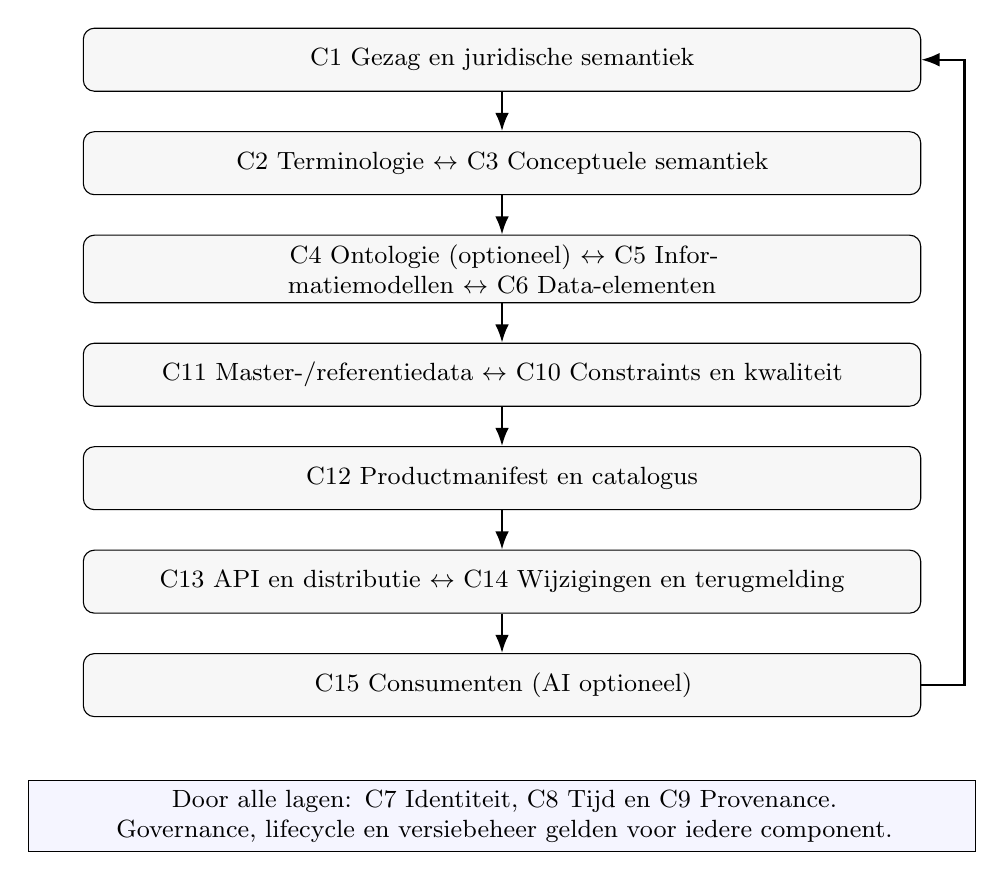
\begin{tikzpicture}[font=\small,box/.style={draw,rounded corners,align=center,text width=10.4cm,minimum height=8mm,fill=black!3},flow/.style={-{Latex},thick}]
\node[box] (a) {C1 Gezag en juridische semantiek};
\node[box,below=5mm of a] (b) {C2 Terminologie $\leftrightarrow$ C3 Conceptuele semantiek};
\node[box,below=5mm of b] (c) {C4 Ontologie (optioneel) $\leftrightarrow$ C5 Informatiemodellen $\leftrightarrow$ C6 Data-elementen};
\node[box,below=5mm of c] (d) {C11 Master-/referentiedata $\leftrightarrow$ C10 Constraints en kwaliteit};
\node[box,below=5mm of d] (e) {C12 Productmanifest en catalogus};
\node[box,below=5mm of e] (f) {C13 API en distributie $\leftrightarrow$ C14 Wijzigingen en terugmelding};
\node[box,below=5mm of f] (g) {C15 Consumenten (AI optioneel)};
\foreach \s/\t in {a/b,b/c,c/d,d/e,e/f,f/g}\draw[flow] (\s)--(\t);
\node[draw,align=center,text width=11.8cm,below=8mm of g,fill=blue!4] (cross) {Door alle lagen: C7 Identiteit, C8 Tijd en C9 Provenance.\\Governance, lifecycle en versiebeheer gelden voor iedere component.};
\draw[flow] (g.east)--++(.55,0)|-(a.east);
\end{tikzpicture}
\caption{Voorgestelde logische reference architecture. Pijlen tonen informatieafhankelijkheden en terugkoppeling; zij claimen geen bestaande implementatie of gemeten gedrag.}
\label{fig:architecture}
\end{figure}

\subsection{Formele beschrijving van het conceptuele metamodel}
Het volgende model is een eigen ontwerpspecificatie; de symbolen zijn geen nieuw gepubliceerde standaard. Een SMDP-release wordt gedefinieerd als:
\[
\mathcal{P}_v=(G_v,\mathcal{D}_v,\mathcal{S}_v,\mathcal{K}_v,\mathcal{Q}_v,\mathcal{B}_v),
\]
waar $G_v$ de semantische verbindingsgraaf is, $\mathcal{D}_v$ verwijzingen naar datasetversies bevat, $\mathcal{S}_v$ diensten en representaties identificeert, $\mathcal{K}_v$ het productcontract beschrijft, $\mathcal{Q}_v$ regels en beschikbare kwaliteitsmetingen bevat en $\mathcal{B}_v$ beheer- en toepasselijkheidsbesluiten vastlegt. Een verwijzing mag naar een externe bron wijzen. Versie $v$ identificeert de release, niet automatisch dezelfde versie voor alle afhankelijke artefacten.

Het gereviseerde graafmodel is $G_v=(N,L,E,\tau,\gamma,\kappa)$, met resourceknopen $N$, literalwaarden $L$ en afzonderlijk geïdentificeerde beweringen/verbindingen $E$. De typering $\tau:N\rightarrow\mathcal{P}(\mathcal{T})$ staat meerdere representatierollen toe. De incidentiefunctie $\gamma:E\rightarrow N\times R\times(N\cup L)$ geeft inhoud en relatietype; $\kappa:E\rightarrow K$ bindt iedere verbinding aan een contextrecord. Twee edges met dezelfde inhoud mogen dus verschillende bronnen, versies en gezagsclaims hebben. Ontbrekende contextwaarden krijgen expliciet de status onbekend; zij verdwijnen niet door samenvoeging van triples. De verzameling typen omvat minimaal:
\begin{align*}
\mathcal{T}=\{&\text{Bron, Gezagsclaim, Term, Definitie, Concept, Klasse,}\\
&\text{Objecttype, Attribuut, DataElementConcept, DataElement,}\\
&\text{ConceptueelDomein, WaardeDomein, Identifier, Entiteitsreferentie,}\\
&\text{Record, Bewering, Dataset, Dienst, Distributie, Product,}\\
&\text{Mapping, Versie, Activiteit, Agent, Regel, Meting, Event, Besluit}\}.
\end{align*}
Een \emph{Entiteitsreferentie} is een representatie van de bedoelde domeinreferent; het model pretendeert niet de werkelijkheid zelf op te slaan. Een \emph{Klasse}-rol en een \emph{Concept}-rol blijven onderscheiden. Zij kunnen in een implementatie afzonderlijke identifiers krijgen, of onder expliciet profielbeleid door dezelfde resource worden gedragen; uit meervoudige typering volgt geen ongedocumenteerde model-equivalentie.

De volgende relatiehandtekeningen leggen de centrale typegrenzen vast:
\begin{align*}
\operatorname{duidtAan}&:\text{Term}\rightarrow\text{Concept},\\
\operatorname{definieert}&:\text{Definitie}\rightarrow\text{Concept},\\
\operatorname{steuntOp}&:\text{Definitie}\rightarrow\text{Bron},\\
\operatorname{formaliseert}&:\text{Klasse}\rightarrow\text{Concept},\\
\operatorname{modelleert}&:\text{Objecttype}\rightarrow\text{Concept},\\
\operatorname{heeftAttribuut}&:\text{Objecttype}\rightarrow\text{Attribuut},\\
\operatorname{representeert}&:\text{DataElement}\rightarrow\text{DataElementConcept},\\
\operatorname{beschrijft}&:\text{Record}\rightarrow\text{Entiteitsreferentie},\\
\operatorname{ontsluit}&:\text{Dienst}\rightarrow\text{Dataset},\\
\operatorname{omvat}&:\text{Product}\rightarrow(\text{Dataset}\cup\text{Dienst}).
\end{align*}
Dit zijn schemahandtekeningen voor relaties, geen totale functies: een term kan contextafhankelijk meerdere concepten aanduiden, en een dataset kan meerdere diensten hebben. Relaties tussen attributen, data-elementconcepten, begrippen en klassen krijgen een Mapping-knoop zodra equivalentie, transformatie of verlies moet worden verantwoord. De relatie \emph{formaliseert} betekent een gemotiveerde formalisatie, niet dat alle juridische nuances behouden zijn.

Een mapping wordt vastgelegd als:
\[
 m=(s,v_s,t,v_t,r,c,j,\ell,a,\sigma),
\]
met bron $s$, bronversie $v_s$, doel $t$, doelversie $v_t$, relatietype $r$, context $c$, rechtvaardiging $j$, bekend betekenisverlies $\ell$, beoordelaar $a$ en status $\sigma$. Mogelijke relatietypen onderscheiden conceptuele overeenkomst, specialisatie, representatietransformatie en vastgestelde co-identiteit. Zij worden niet allemaal op één bestaande RDF-property afgebeeld. Bij publicatie moet per type worden gekozen of SKOS, OWL, PROV-O of een gemotiveerde uitbreiding past. \citep{S31,S30,S33}

Een bewering krijgt afzonderlijke context:
\[
 b=(id_b,s,p,o,\iota_v,\iota_r,z,\pi,\epsilon),
\]
waar $id_b$ de afzonderlijke beweringsidentiteit is, $s,p,o$ de inhoud aanduiden, $\iota_v$ het geldigheidsinterval, $\iota_r$ het registratie-interval in systeem $z$, $\pi$ de provenanceverwijzing en $\epsilon$ de epistemische metadata. Publicatie- en eventtijd worden apart toegevoegd aan respectievelijk distributie en event. De bitemporele onderscheiding is gebaseerd op Jensen et al.; OWL-Time en PROV-O zijn representatiekandidaten voor onderdelen van de context. \citep{L14,S37,S33}

De epistemische annotatie is als eigen profiel gedefinieerd door:
\[
\epsilon=(k,r_g,m,u,g,e,a),
\]
met uitspraaksoort $k$, registratiehandeling $r_g$, productiemethode $m$, onzekerheidsbeschrijving $u$, gezagsgrond $g$, bewijsstatus $e$ en verantwoordelijke $a$. Registratie en afleiding kunnen samen voorkomen. De methode vermeldt bijvoorbeeld menselijke invoer, een berekeningsregel of een geïdentificeerd AI-model; zij maakt geen kansuitspraak. Een AI-methode is niet per definitie een gekalibreerd probabilistisch model. $u$ kan afwezig, onbekend of methodisch beschreven zijn; een getal krijgt alleen een probabilistische interpretatie als die interpretatie is onderbouwd. $g$ onderscheidt wettelijke authenticiteit van ander gezag. $e$ onderscheidt onbeoordeeld, ondersteund, betwist en ingetrokken bewijs. Deze waarden zijn ontwerpkeuzen, geen PROV-O-enumeraties.

Een contextrecord $K$ bindt daarnaast de bronversie, het perspectiefsysteem en relevante model-/mappingversies. Voor bekende tijdsgrenzen wordt de conventie $[begin,einde)$ gekozen. Een open einde en een onbekende grens zijn afzonderlijke toestanden; onbekend is niet oneindig geldig. Een gedeeltelijk geïnterpreteerde relatie kan daardoor geen tweewaardige waarheidsbeslissing afdwingen. De voorlopige controle levert \emph{voldoet}, \emph{schendt} of \emph{onbepaald}; ontbrekende verplichte metadata is een contractschending, maar de inhoudelijke waarheid van het gegeven kan alsnog onbepaald zijn.

\paragraph{Analytisch tegenvoorbeeld, niet uitgevoerd.}
Neem twee synthetische beweringen $b_1$ en $b_2$ met dezelfde inhoud $(x,p,7)$, maar bron A respectievelijk bron B. Alleen A heeft een beoordeelde gezagsgrond. Dan mogen $id_{b_1}$ en $id_{b_2}$ niet door deduplicatie verdwijnen: gelijkheid van waarde impliceert geen gelijkheid van context. Een latere versie $b_3$ corrigeert A naar waarde 8 met terugwerkende geldigheid. Een bekend-op-vraag vóór de correctieregistratie selecteert de eerdere bronversie; een latere bekend-op-vraag selecteert de correctie voor zover de geldigheidsvraag dat vereist. Deze verwachte uitkomst volgt uit het voorgestelde contract, niet uit een gedraaide prototypequery. Een verdedigbare alternatieve implementatie bewaart dezelfde informatie in relationele bewerings- en contexttabellen.

\subsection{Voorgestelde invarianten}
De volgende invarianten operationaliseren de requirements en moeten later in constraints en evaluatiescenario’s worden vertaald.

\begin{enumerate}[label=I\arabic*.,leftmargin=1cm]
\item \textbf{Typegrens.} Geen impliciete gelijkheid tussen term, concept, klasse, modelelement, record en referent. Een overgang vereist een getypeerde relatie (R01/R11).
\item \textbf{Gezagsbewijs.} Iedere gepubliceerde positieve authenticiteitsclaim verwijst naar een vastgelegde grondslag, toepassingscontext en verantwoordelijkheidsbesluit; ontbreken wordt als onbekend zichtbaar (R02/R08/R23).
\item \textbf{Identiteit.} Een identifier heeft een beheerde scope en referentsoort. Een wijziging van label of document-URL verandert niet zonder identiteitsbesluit de referent (R03).
\item \textbf{Historie.} Een correctie creëert een nieuw registratiekennisinterval en bewaart de eerdere versie voor zover het toepasselijke bewaarbeleid dat toestaat. Geldigheid en registratie worden niet uit één ongetypeerd tijdveld afgeleid (R06/R20).
\item \textbf{Afleiding.} Een afgeleid gegeven verwijst naar invoerversies, activiteit en regel- of modelversie voor zover beschikbaar; ontbrekende noodzakelijke context wordt expliciet als contractafwijking gepubliceerd. Afleiding erft niet automatisch wettelijke authenticiteit (R07/R23).
\item \textbf{Validatiebereik.} Een validatie-uitkomst vermeldt datasetversie, shapeversie en redeneerconfiguratie. Conformiteit wordt niet als werkelijkheidsbewijs gepubliceerd (R09/R16).
\item \textbf{Releasebinding.} Een productrelease verwijst naar vastgelegde versies van definities, modellen, mappings, contexten, regels en interfaces, of documenteert expliciet welke afhankelijkheid dynamisch blijft (R10/R13).
\item \textbf{Wijzigingsbetekenis.} Een event verwijst naar een identificeerbare bron en opvraagbare wijzigingscontext. Ontvangstvolgorde alleen bepaalt niet de geldigheidsvolgorde (R15).
\end{enumerate}
Een invariant is niet automatisch in SHACL volledig afdwingbaar. Type- en verwijzingscontroles kunnen vaak als graafconstraints worden voorgesteld; een juridische grondslag of correcte identiteitsbeslissing vergt daarnaast deskundige beoordeling. Dit onderscheid volgt uit de scope van SHACL als graafvalidatie. \citep{S32}

\subsection{Interfaces en informatiestromen}
De architectuur definieert logische interfacecontracten, geen bestaande endpoints. Tabel~\ref{tab:interfaces} benoemt wat over componentgrenzen moet worden uitgewisseld. Protocolkeuze volgt pas uit toepasselijkheid en implementatiebesluit.

\begin{longtable}{@{}P{.10\linewidth}P{.25\linewidth}P{.56\linewidth}@{}}
\caption{Voorgestelde interfaces en informatiecontracten.}\label{tab:interfaces}\\
\toprule Interface & Componenten & Contract \\ \midrule\endfirsthead
\toprule Interface & Componenten & Contract \\ \midrule\endhead
IF1 & C1--C6 & Semantische registratie: getypeerde resource, bron, versie, context, reviewstatus en onderlinge mapping; geen automatische publicatie na import. \\
IF2 & C7--C9 naar alle lagen & Contextresolutie: scoped identifier, versie, tijdas, provenance en epistemische status; ontbrekend bewijs expliciet teruggeven. \\
IF3 & C11 naar C9/C10/C12 & Bronopname: recordversie, schema, tijdcontext en bronverwijzing; validatierapport blijft afzonderlijk van de inhoud. \\
IF4 & C10 naar C12 & Vrijgave-informatie: getoetste regels, meetpopulatie, resultaat, openstaande afwijkingen en verantwoordelijke voor acceptatie. \\
IF5 & C12 naar C13/C15 & Productmanifest: doel, gebruikscondities, datasets/diensten, semantische versies en gepubliceerde kwaliteits- en bewijsbeperkingen. \\
IF6 & C14 naar C13/C15 & Verandering: eventidentiteit, bronobject, oude/nieuwe versie waar beschikbaar, changetype en herstelverwijzing. \\
IF7 & C15/C13 naar C14/C1/C11 & Terugmelding: betwiste uitspraak, bewijs, indienerrol, status en bronhouderroute; melding wijzigt niet vanzelf het bronrecord. \\
\bottomrule
\end{longtable}

Een voorgestelde publicatiestroom begint met een gecontroleerde definitiebron in C1/C2. C3--C6 leggen vervolgens concept, ontologische keuze, modelconstructie en data-element vast. C11 verbindt bronrecords met deze beschrijvingen; C7--C9 leveren identiteit, tijdcontext en provenance. C10 voert de overeengekomen controles uit. C12 publiceert daarna een manifest op basis van een bevoegd vrijgavebesluit. C13 en C14 leveren representaties en notificaties; C15 maakt de context beschikbaar aan afnemers. Deze volgorde beschrijft een mogelijke gecontroleerde release, geen veronderstelde bestaande workflow.

Een tweede stroom betreft semantische wijziging zonder recordwijziging. Een herziene definitie kan een mapping of shape beïnvloeden terwijl de bronwaarden identiek blijven. De afhankelijkhedengraaf moet dergelijke impact zichtbaar maken. Een derde stroom betreft een retrospectieve correctie: het bronrecord krijgt een nieuwe registratieversie, de geldigheid wordt afzonderlijk bijgewerkt en een event verwijst naar de correctie. Een vierde stroom betreft afleiding: een AI-uitspraak krijgt een eigen activiteit en status en wordt niet zonder besluit teruggeschreven als authentiek brongegeven.

\subsection{Normatieve en afgeleide informatie}
Normatieve definities en toepasselijke regels worden als brongebonden uitspraken beheerd; de semantische representatie is een interpretatie daarvan wanneer zij niet rechtstreeks door de bevoegde bron is vastgesteld. Een OWL-axioma dat een wettelijke tekst formaliseert, krijgt daarom een verantwoordelijke en een beoordelingsstatus. Een afgeleid record verwijst naar zowel invoer als gebruikte interpretatieversie. De architectuur verplaatst het institutionele gezag niet naar de technische graaf.

Voor machineconsumenten wordt een \emph{interpretatiepakket} voorgesteld: de aangevraagde gegevens met relevante definities, identifiers, model-/mappingversies, provenance, kwaliteitsuitkomsten en epistemische beperkingen. Het pakket hoeft niet alle metadata integraal in elk antwoord te kopiëren; vaste verwijzingen met een afgesproken resolutiecontract zijn een alternatief. Of deze vorm bruikbaar en efficiënt is, moet de evaluatie vaststellen.

\subsection{Governance, lifecycle en versiebeheer}
De voorgestelde governance onderscheidt de bronverantwoordelijke, begripsbeheerder, model-/mappingbeheerder, producteigenaar en afnemer. Een juridische deskundige beoordeelt gezags- en toepasselijkheidsclaims waar nodig. Functies kunnen organisatorisch samenvallen, maar besluiten en rollen blijven traceerbaar. Deze inrichting is een synthese van registratiebeheer, BOMOS en governance\-onderzoek. \citep{S10,S23,L07}

De lifecycle luidt als ontwerpvoorstel: concept, review, vastgesteld, gepubliceerd, verouderd en ingetrokken. Herziening creëert een nieuwe versie met een relatie tot de vorige; intrekking wordt zichtbaar in resolutie en catalogus. Publicatie vereist een expliciet vrijgavebesluit. Compatibiliteit wordt niet afgeleid uit een versienummer alleen: een definitiewijziging kan semantisch brekend zijn zonder syntactische schemawijziging. Het manifest legt daarom afhankelijkheden en compatibiliteitsbesluiten vast.

Voor een release $v$ definieert het manifest een afhankelijkhedenverzameling $D(v)=\{(a_i,v_i,c_i)\}$ met artefact, gekozen versie en compatibiliteitsbesluit. De evaluatie moet toetsen of dezelfde release daarmee opnieuw kan worden geïnterpreteerd. Waar een dynamische bron geen vaste snapshot toelaat, wordt die beperking gepubliceerd in plaats van reproduceerbaarheid te suggereren. Bewaar- en verwijderbeleid worden afzonderlijk beoordeeld; versiebeheer impliceert geen onbeperkte bewaring van alle gegevens.

\subsection{Minimale realisatie en concurrerende architecturen}
De minimale realisatie heeft vijf functies: (1) bron- en begripsregistratie, (2) contextbinding bij beweringen, (3) een versiegebonden productmanifest, (4) een distributiecontract en (5) review/validatie van wijzigingen. Deze functies kunnen in één conventionele database en applicatie worden gerealiseerd. C1--C15 zijn views op die functies. C4 vereist alleen een expliciete beoordeling van de ontologische keuze; zonder concrete behoefte hoeft geen zelfstandige ontologie te worden gebouwd. C14 wordt geactiveerd bij notificatievereisten; C15 is een afnemerscontract en geen verplichte AI-voorziening.

\begin{longtable}{@{}P{.23\linewidth}P{.34\linewidth}P{.35\linewidth}@{}}
\caption{Ontwerpalternatieven; de keuze is nog niet empirisch beslist.}\\
\toprule Variant & Reden om te onderzoeken & Mogelijke reden voor verwerping \\ \midrule
A1: conventioneel contextregister & Dezelfde feiten, context en versiehistorie via tabellen, documentverwijzingen en vaste rapporten; sterke eenvoudiger comparator. & Als expliciete koppelingen een vooraf relevante interpretatiewinst leveren die niet even goedkoop met A1 wordt bereikt. \\
B1: getypeerd contextbindingsprofiel & Expliciete edge-identiteit, mappings en afhankelijkheden; RDF is een mogelijke publicatierepresentatie. & Bij praktische gelijkwaardigheid van A1, hogere beheerkosten of meer fouten door contextselectie. \\
B2: B1 plus ontologische verdieping & Aanvullende axioma’s of UFO/OntoUML-review bij aangetoonde identiteit-/rolproblemen. & Als detectiewinst de extra analyse- en onderhoudsinspanning niet rechtvaardigt. \\
\bottomrule\end{longtable}

Bestaand semantisch MDM-werk en kennisgraaftechnieken maken plausibel dat verschillende fysieke realisaties mogelijk zijn. \citep{L18,L13} Zij kiezen de winnaar niet. DPROD is een kandidaat om C12-inhoud te hergebruiken; een nieuw productschema wordt alleen voorgesteld waar de gekozen bron- en taakcontext een aantoonbare aanvulling vraagt. \citep{S51}

Centralisatie wordt onafhankelijk van representatie gekozen. Een centraal besluitpunt kan conflicterende belangen verhullen; federatie kan afhankelijkheden en resolutiestoringen toevoegen. Beide zijn ontwerp-risicoscenario’s, geen gemeten incidenten. C1 registreert daarom het bestaan van geschillen en bevoegde besluiten; het kiest niet automatisch één universele definitie. Voor toegang geldt hetzelfde beginsel: een onbereikbare of ingetrokken bron wordt niet als lege of inhoudelijk onjuiste bron behandeld. Het contract legt vast welke context de afnemer daadwerkelijk mocht ontvangen.

\section{Design Principles}
\label{sec:principles}
De principes hieronder zijn ontwerpkennis in voorstelvorm. MOET en ZOU drukken sterkte binnen het voorgestelde profiel uit. De rationale verbindt bronkennis met het ontwerpprobleem; het testonderdeel specificeert toekomstige beoordeling van het prototype. Het bestaan van ondersteunende bronnen maakt de principes niet empirisch gevalideerd.

\subsection*{DP1 --- Expliciete typen en gemotiveerde mappings}
\textbf{DP1.} Een Semantic Master Data Product MOET termen, begrippen, definities, ontologische klassen, modelelementen, data-elementen, entiteiten, records en producten als onderscheiden rollen typeren en hun verbindingen expliciet maken. Afzonderlijke fysieke resources zijn niet in alle gevallen vereist.

\textbf{Rationale.} ISO 704, SKOS, MIM en ISO/IEC 11179 beschrijven verschillende eenheden. \citep{S11,S31,S13,S08} Een gedeeld label of technisch veld geeft geen volledige onderbouwing van equivalentie. ISO 8000-110 motiveert bovendien aandacht voor semantic encoding en dataspecificatie, zonder hier een specifieke technologie af te dwingen. \citep{S03} De ontwerpkeuze is daarom een getypeerde verbinding in plaats van stilzwijgende samenvoeging.

\textbf{Gerelateerde standaarden en eisen.} ISO 704, NL-SBB/SKOS, MIM, ISO/IEC 11179, ISO 8000-110 en OWL; R01, R04, R05 en R11. \textbf{Te testen in prototype.} M01, M04, M05 en M11 moeten typeverwarring, ontbrekende data-elementkoppelingen en onterechte equivalenties detecteren. De prototypeanalyse zal toetsen of mappings een versie en besluitgrond hebben.

\subsection*{DP2 --- Gezag en bewijs op het niveau van de uitspraak}
\textbf{DP2.} Een Semantic Master Data Product MOET gezagsclaims en provenance verbinden met de uitspraak en haar context, en MOET technische afzenderidentiteit, wettelijke authenticiteit en feitelijke juistheid onderscheiden.

\textbf{Rationale.} De stelseleisen betreffen institutionele verantwoordelijkheden; PROV-O representeert herkomst; FSC organiseert technische vertrouwensrelaties. \citep{S25,S33,S21} Deze scopes zijn complementair. Het ontwerp voorkomt dat een geauthenticeerde transmissie automatisch de inhoud juridisch kwalificeert. Toepasselijkheid van Europese verplichtingen vraagt eveneens een afzonderlijk oordeel. \citep{S42,S43}

\textbf{Gerelateerde standaarden en eisen.} NL-SBB, PROV-O, ISO 8000-120, FSC, stelseleisen, EIF en Interoperable Europe Act; R02, R07, R08 en R21. \textbf{Te testen in prototype.} M02/M07 toetsen herleidbaarheid, M08 onterechte gezagsclaims en M21 correcte toepasselijkheidsbesluiten. Een correct opgeloste identifier telt niet als vervanging van een ontbrekende rechtsgrond.

\subsection*{DP3 --- Identiteit en versie onafhankelijk van labels}
\textbf{DP3.} Een Semantic Master Data Product MOET identifier-scope en referentsoort vastleggen en MOET versieerbare beschrijvingen onderscheiden van de geïdentificeerde entiteit.

\textbf{Rationale.} URI/IRI-syntax en publicatierichtlijnen lossen andere problemen op dan ontologische identiteit. \citep{S38,S39,L08} Labels en representaties kunnen wijzigen zonder dat dezelfde soort identiteitsbeslissing aan de orde is. Het ontwerp registreert daarom zowel blijvende verwijzing als gewijzigde beschrijving.

\textbf{Gerelateerde standaarden en eisen.} RDF, URI/IRI, Cool URIs, DCAT 3 en ontologische analyse; R03 en R10. \textbf{Te testen in prototype.} M03 toetst uniciteit, scope en resolutie. M10 zal nagaan of een oude release reproduceerbaar blijft en of modelwijzigingen naar de juiste afhankelijke resources worden doorgeleid.

\subsection*{DP4 --- Historisch interpreteerbare uitspraken}
\textbf{DP4.} Een Semantic Master Data Product MOET geldigheid en registratiekennis afzonderlijk modelleren en ZOU bewaarde bewijsobjecten aan het toepasselijke bewaarmetadata-profiel verbinden.

\textbf{Rationale.} De temporele literatuur onderscheidt valid en transaction time; OWL-Time representeert tijdconstructies en PROV-O afleidingscontext. \citep{L14,S37,S33} MDTO kan relevant zijn voor duurzaam te bewaren informatieobjecten, maar is geen universeel historieprofiel voor masterdata. \citep{S24}

\textbf{Gerelateerde standaarden en eisen.} OWL-Time, PROV-O, ISO 8000-120, MDTO en TOOI waar toepasselijk; R06, R07 en R20. \textbf{Te testen in prototype.} M06 toetst retrospectieve correcties en bekend-op-vragen; M07 bronversies; M20 het vooraf afgebakende bewaarprofiel. Ontbrekende bronhistorie wordt als beperking gerapporteerd, niet door schijnprecisie vervangen.

\subsection*{DP5 --- Gescheiden inferentie, validatie en kwaliteitsbeoordeling}
\textbf{DP5.} Een Semantic Master Data Product MOET logische gevolgtrekking, toetsing van beschikbare gegevens en beoordeling van feitelijke kwaliteit als afzonderlijke processen en uitkomsten publiceren.

\textbf{Rationale.} RDFS/OWL, SHACL en kwaliteitsmodellen hanteren verschillende criteria. \citep{S29,S30,S32,S12,L15} DQV maakt metingen beschrijfbaar, maar levert geen casusgebonden grens voor voldoende kwaliteit. \citep{S34} Een geslaagd schema is dus geen toereikende kwaliteitsclaim.

\textbf{Gerelateerde standaarden en eisen.} ISO 8000, ISO/IEC 25012, NORA, RDF/RDFS, OWL, SHACL en DQV; R05, R09 en R16. \textbf{Te testen in prototype.} M05/M09 controleren decodeerbaarheid en meetcontext. M16 vergelijkt constraintdetectie met een onafhankelijk foutencorpus en houdt externe feitelijke beoordeling afzonderlijk.

\subsection*{DP6 --- Productcontract met bereikbare betekenis}
\textbf{DP6.} Een Semantic Master Data Product MOET een versiegebonden contract publiceren dat doel, eigenaar, datasets, diensten, kwaliteit, gebruikscondities en semantische afhankelijkheden machinevindbaar verbindt.

\textbf{Rationale.} Dataproductliteratuur motiveert gebruikersoriëntatie; DCAT-profielen ondersteunen catalogisering; FAIR motiveert machinegericht hergebruik. \citep{L12,S47,S45,S16,L11} De combinatie vereist een eigen contractuitbreiding, waarvan de volledigheid niet uit het bestaan van een catalogusrecord volgt.

\textbf{Gerelateerde standaarden en eisen.} DCAT 3, DCAT-AP(-NL), FAIR, OpenAPI, REST API Design Rules, Digikoppeling, JSON-LD en relevante FDS-afspraken; R13, R14, R17 en R18. \textbf{Te testen in prototype.} M13/M14 toetsen contract en distributie, M18 de toepasselijkheid van FDS-afspraken en M17 of consumenten de juiste betekenis en broncontext vinden. Beschikbaarheid wordt onderscheiden van correct gebruik.

\subsection*{DP7 --- Beheerde verandering en terugmelding}
\textbf{DP7.} Een Semantic Master Data Product MOET semantische en technische wijzigingen, statusovergangen en terugmeldingen verbinden met verantwoordelijke besluiten en herstelbare versiecontext.

\textbf{Rationale.} Registratiebeheer, BOMOS en governance\-onderzoek ondersteunen expliciete verantwoordelijkheden. \citep{S10,S23,L07,L17} Het NL GOV CloudEvents-profiel biedt een notificatievorm, maar bepaalt niet zelfstandig de betekenis van iedere domeinwijziging of het herstelbeleid. \citep{S22}

\textbf{Gerelateerde standaarden en eisen.} ISO/IEC 11179-6, BOMOS, NL GOV CloudEvents, stelseleisen, kwaliteitsbaseline, FDS en conditioneel MDTO; R10, R12, R15, R19 en R20. \textbf{Te testen in prototype.} M10/M12 toetsen afhankelijkheden en bevoegdheden; M15 duplicaten, volgorde en herstel; M19 terugmeldsporen; M20 bewaarcontext. Een gepubliceerd event wordt niet als bewijs van succesvolle verwerking bij iedere afnemer beschouwd.

\subsection*{DP8 --- Ontologische verdieping naar aantoonbare behoefte}
\textbf{DP8.} Een Semantic Master Data Product ZOU ontologische analyse toepassen wanneer identiteit, rollen, fasen of afhankelijkheden tot relevante interpretatieverschillen leiden, en MOET de gemaakte keuze en extra inspanning verantwoorden.

\textbf{Rationale.} UFO/OntoUML en OntoClean bieden conceptuele analysemiddelen, maar het dossier toont geen universele meerwaarde voor overheidsregistraties. \citep{L08,L09,L10,S40,S41} De architectuur laat daarom zowel beperkte als uitgebreidere ontologische uitwerking toe.

\textbf{Gerelateerde standaarden en eisen.} MIM, OWL en SKOS als aangrenzende representaties; UFO/OntoUML en OntoClean als methodische opties, niet als Nederlandse overheidsstandaarden; R11 en R22. \textbf{Te testen in prototype.} M11/M22 vergelijken gedetecteerde mapping- en categoriefouten, fout-positieven en analistentijd met een MIM-gebaseerde analyse zonder aanvullende foundational ontology.

\subsection*{DP9 --- Expliciete epistemische status voor machineconsumenten}
\textbf{DP9.} Een Semantic Master Data Product MOET uitspraaksoort, registratiehandeling, productiemethode, onzekerheidsbeschrijving, gezagsgrond en bewijsstatus afzonderlijk machineleesbaar maken en MOET onbekend of betwist bewijs zichtbaar houden.

\textbf{Rationale.} PROV-O, stelselgezag en FAIR bieden afzonderlijke bouwstenen. \citep{S33,S25,L11} De samengestelde classificatie is een eigen voorstel. Retrievalonderzoek toont geen rechtvaardiging om AI-uitkomsten automatisch als gezaghebbende feiten te publiceren. \citep{L16}

\textbf{Gerelateerde standaarden en eisen.} PROV-O, ISO 8000-120 en FAIR, met expliciete aansluiting op gezagsbesluiten; R08, R17 en R23. \textbf{Te testen in prototype.} M23 toetst of deskundigen en consumenten de categorieën correct onderscheiden. M17/M08 toetsen brongebonden antwoorden en onterechte opwaardering. De evaluatie moet vaststellen of de annotaties interpretatiefouten verminderen; hun aanwezigheid alleen volstaat niet.

\section{Casus Stelsel van Basisregistraties}
\subsection{Onderbouwde casusgrens}
De primaire casus is het Stelsel, maar het beschikbare dossier ondersteunt slechts een beperkte concrete objectselectie uit de BAG: nummeraanduiding, verblijfsobject en pand. De geregistreerde officiële BAG-catalogusbron dient als grondslag voor deze selectie. \citep{S49} Het dossier biedt onvoldoende vastgelegde primaire inhoud om een volledige juridisch gevalideerde keten met persoon, perceel en WOZ-object te modelleren. Daarom worden geen BRP-, BRK- of WOZ-definities, cardinaliteiten of identiteitsregels ingevuld op basis van veronderstellingen.

Dit beperkt de bewijskracht wezenlijk: een BAG-fragment is geen empirische demonstratie van interoperabiliteit tussen basisregistraties. De nog niet gevalideerde onderzoeksroute wordt als toekomstig uitbreidingsontwerp weergegeven:
\begin{center}
\small
persoon $\dashrightarrow$ adres/nummeraanduiding $\dashrightarrow$ verblijfsobject\\
$\dashrightarrow$ pand $\dashrightarrow$ perceel $\dashrightarrow$ WOZ-object.
\end{center}
De gestippelde pijl betekent hier uitsluitend ``te onderzoeken verbinding'', geen vastgestelde registratierelatie, navigatiepad of cardinaliteit. Ook het gebruik van \emph{adres} als knoop moet worden onderzocht: een beschrijving, een samengesteld gegeven en een registratieobject mogen niet stilzwijgend gelijkgesteld worden.

\subsection{Analytische toepassing op het BAG-fragment}
Voor de drie geselecteerde objectcategorieën stelt het ontwerp dezelfde onderzoekseenheid voor: een conceptbeschrijving, een eventuele ontologische klasse, een modeltype, data-elementen en verwijzingen naar recordversies. De categorieën worden niet samengevoegd omdat een applicatie ze gezamenlijk presenteert. De catalogus ondersteunt hun keuze als domeinonderwerpen; de concrete relaties en hun juridische gevolgen moeten later uit volledige gecontroleerde inhoud worden overgenomen. \citep{S49}

\begin{longtable}{@{}P{.22\linewidth}P{.40\linewidth}P{.30\linewidth}@{}}
\caption{Voorgestelde casusvragen; geen reeds uitgevoerde casustoets.}\\
\toprule Aspect & Vraag voor het BAG-fragment & Benodigde aanvulling vóór evaluatie \\ \midrule\endfirsthead
\toprule Aspect & Vraag voor het BAG-fragment & Benodigde aanvulling vóór evaluatie \\ \midrule\endhead
Begrip en definitie & Welke afzonderlijke begrippen worden bedoeld en welke bronversie begrenst ze? & Geverifieerde definitietekst en toepassingscontext per categorie. \\
Identiteit & Welke identifier verwijst naar object, record, versie of document? & Officieel uitgifte-, scope- en historiebeleid; geen afleiding uit tekenreekslengte alleen. \\
Relaties en modellen & Welke relaties bestaan en welke betekenis behouden modeltransformaties? & Vastgestelde modelelementen, rollen en cardinaliteiten; gereviewde MIM/OWL-mapping. \\
Ontologische verschillen & Wordt een fysieke, administratieve of andere referent gemodelleerd en welke identiteit geldt? & Domeindeskundige beoordeling; een UFO-classificatie blijft een gemotiveerd voorstel. \\
Provenance en gezag & Welke bron ondersteunt welke waarde en authenticiteitsclaim? & Attribuut-/uitspraakgebonden grondslag en bronrecordversie. \\
Historie & Welke situatie gold wanneer en welke versie was toen bekend? & Brongebonden definitie van tijdvelden en beschikbaarheid van historie. \\
Koppeling buiten BAG & Is er identiteit, gedeeltelijke overlap of slechts een functionele relatie? & Primaire BRP/BRK/WOZ-bronnen, bevoegdheidsbeoordeling en afzonderlijke mappingvalidatie. \\
\bottomrule
\end{longtable}

Een synthetisch scenario kan later een correctie van een eerder gepubliceerd gegeven gebruiken. De juiste uitkomst hangt dan af van zowel de geldigheidsdatum als het registratiemoment bij de gekozen bron. Een tweede scenario kan twee gelijknamige velden uit verschillende modelversies vergelijken. Een derde scenario kan een AI-afgeleide correspondentie aanbieden waarvoor geen bevoegde bevestiging bestaat. Deze scenario’s zijn ontworpen foutprikkels, geen gerapporteerde gebeurtenissen in de BAG. Een Stelselbrede effectclaim is pas toelaatbaar na brongecontroleerde evaluatie van minimaal twee onafhankelijk beheerde registraties met inhoudelijk verschillende identiteits- of tijdscontext. Twee registraties zijn een minimale stage-gate, geen bewijs van representativiteit voor het hele Stelsel.

\subsection{Criteria voor uitbreiding naar meerdere registraties}
Een uitbreiding wordt pas in de empirische casus opgenomen wanneer per relatie de primaire bron, definitie, identifier-scope, tijdsbetekenis, gezagsgrond en toegestane verwerking zijn vastgesteld. Het onderzoeksprotocol moet bovendien voldoende negatieve voorbeelden bevatten: gelijke labels zonder equivalentie, gedeeltelijke overlap en wijzigingen waarbij object- en recordidentiteit uiteenlopen. De meerregistratieclaim blijft tot die uitbreiding onbewezen. Gebruik van openbare informatie wordt niet gelijkgesteld aan onbeperkte herbruikbaarheid van alle mogelijke persoonsgegevens; een concrete verwerking vergt een afzonderlijke beoordeling die buiten deze paper valt.

\section{Bestaand prototype}
Het bestaan van een technisch prototype is onderzoekscontext op basis van de opdracht. De huidige repository bevat het onderzoeksdossier; daarin zijn geen prototypebroncode, deploymentbeschrijving, versie-identificatie, testrapporten of geverifieerde implementatiemapping opgenomen. Deze lokale inventarisatie rechtvaardigt geen uitspraak over welke technologieën of standaarden het prototype daadwerkelijk implementeert.

Er wordt daarom geen implementatiearchitectuur getekend alsof zij is vastgesteld. De reference architecture is een voorstel waarmee het prototype later vergeleken zal worden. Voorafgaand aan die vergelijking moeten repositorylocatie, commit of release, configuratie, gegevensselectie, modelversies, afhankelijkheden en bekende beperkingen worden geregistreerd. Elke feitelijke component krijgt vervolgens een mapping naar C1--C15 met de status aanwezig, gedeeltelijk aanwezig, afwezig of nog niet beoordeeld. Het ontbreken van die inventarisatie is op dit moment een bewijsgrens, geen vastgesteld gebrek van het prototype.

De prototype-evaluatie zal eisen uit de literatuur toetsen via R01--R23: onder meer typezuiverheid, brongebonden definities, identifier-scope, bitemporale reconstructie, provenance, toetsbare kwaliteitsregels, versiegebonden mappings, productcontracten, wijzigingen en epistemische status. Bestaande implementatiekeuzen mogen bij deze toets niet achteraf de criteria bepalen. Een wijziging van het prototype tijdens een formatieve fase krijgt een nieuwe versie; een summatieve test vereist vooraf bevroren criteria en artefactversie.

\section{Voorgestelde evaluatiemethode}
\label{sec:evaluation}
\subsection{Evaluatievragen, eenheden en episodes}
De evaluatie moet vaststellen of het ontwerp bruikbaar, uitvoerbaar en semantisch adequaat is, en welke extra kosten het veroorzaakt. FEDS ondersteunt het onderscheiden van verschillende evaluatiedoelen en contexten. \citep{L03} De volgende vier episodes zijn eigen operationaliseringen.

In een eerste, formatieve episode beoordelen onafhankelijke deskundigen requirements, begrippen, mappings en juridische toepasselijkheidsbesluiten. Hun opmerkingen leiden tot gereviseerde ontwerpversies, niet tot een summatieve effectclaim. In een tweede, kunstmatige episode worden gecontroleerde fout-, wijzigings- en historiescenario’s uitgevoerd tegen een bevroren prototypeversie. Een derde episode vergelijkt menselijke interpretatie en wijzigingsanalyse in taakgerichte sessies. Een vierde episode onderzoekt machineconsumptie, inclusief een afzonderlijke AI-taakset. Een latere praktijkepisode met bronhouders en afnemers moet de ecologische geldigheid toetsen.

De analyse-eenheden zijn niet onderling uitwisselbaar: een metadataresource, mappingpaar, bewering, wijzigingsscenario, gebruikstaak en deelnemer vragen elk een eigen noemer. Herhaalde antwoorden van hetzelfde model op dezelfde vraag zijn geen onafhankelijke domeincases. De datasetselectie en analyse-eenheden worden vóór de summatieve fase vastgelegd.

\subsection{Sterke comparatoren en afzonderlijke interventies}
Het primaire experiment onderscheidt A0, A1 en B1. A0 biedt technische masterdata en gangbare documentatie; A1 biedt dezelfde inhoud als B1, inclusief bronverwijzingen, tijdinformatie, gezagsbesluiten en beschikbare kwaliteitsinformatie in een conventioneel contextregister. B1 voegt de expliciete getypeerde contextbinding en machinevolgbare afhankelijkheden toe. A1 mag gestructureerde velden, SQL, zoekfuncties en rapportages gebruiken; het wordt niet kunstmatig verzwakt. Als A1 hetzelfde contract eenvoudig kan realiseren, is dat een relevante uitkomst tegen de noodzaak van B1.

De inhoud wordt vóór uitvoering vergeleken met een informatie-inventaris. Taakrelevante feiten die alleen B1 bezit worden óf aan A1 toegevoegd óf als apart pakketverschil geanalyseerd. Toegang, presentatie, zoekmogelijkheden, antwoordbudget en training worden zo gelijk mogelijk gehouden. Waar gelijkstelling niet mogelijk is, wordt het overblijvende verschil onderdeel van de interventiedefinitie. A0--B1 meet hooguit pakketwaarde; A1--B1 is de primaire toets van aanvullende contextbinding. Er wordt geen zuiver ``effect van RDF'' geclaimd wanneer tegelijk interface, tooling of verwerking verandert.

Een voorafgaande manipulatiecheck specificeert welke contextverbindingen B1 automatisch volg- en versieerbaar maakt en hoe A1 dezelfde informatie aanbiedt. Als de twee implementaties een gelijkwaardig contract en dezelfde bewerkingsmogelijkheden bieden, ontbreekt een onderscheidende semantische interventie. Het onderzoek mag dan alleen implementatiekosten/-prestaties vergelijken; een vermeend uniek SMDP-mechanisme is niet geïdentificeerd. Deze uitkomst moet vóór een causale effectclaim worden gerapporteerd.

De aanvullende ontologievariant B2 wordt afzonderlijk onderzocht. Epistemische annotatievorm en annotatiebetrouwbaarheid worden in een aparte episode gemanipuleerd. Daardoor kan een voordeel aan een specifieker mechanisme worden gerelateerd in plaats van aan alle standaarden tegelijk. De evaluatie volgt de DSR-onderscheiding tussen formatieve aanpassing en summatieve toets; de definitieve vergelijkingen worden vóór de laatste fase vastgezet. \citep{L03}

\subsection{Experimenten, variabelen en estimands}
\begin{longtable}{@{}P{.08\linewidth}P{.27\linewidth}P{.30\linewidth}P{.27\linewidth}@{}}
\caption{Geplande experimenten. Geen condities zijn uitgevoerd of resultaten verzameld.}\label{tab:experiments}\\
\toprule ID & Onafhankelijke variabele & Primaire afhankelijke variabele & Controle en grens \\ \midrule\endfirsthead
\toprule ID & Onafhankelijke variabele & Primaire afhankelijke variabele & Controle en grens \\ \midrule\endhead
E1 & Representatie A0/A1/B1; taaktype identiteit/tijd/gezag. & Aandeel inhoudelijk correcte én geldig herleidbare antwoorden; verschil B1--A1. & Gelijke informatie, toegang en training; tijd en kosten apart; gestratificeerde taken. \\
E2 & Annotatievorm conventioneel/expliciet, gekruist met juiste, ontbrekende of misleidende statusinformatie. & Onterechte gezagsopwaarderingen per beoordeelde uitspraak; correcte en onnodige onthouding. & Dezelfde bewijsinhoud per kwaliteitsniveau; mens en AI apart; geen werkelijke incidentclaim. \\
E3 & Modelreview zonder/met gerichte ontologische verdieping. & Extra juist gedetecteerde identiteit-/rolfouten én analistentijd. & Gelijke taakset en expertise; fout-positieven apart; geen labels met het correcte antwoord in de taak. \\
E4 & Zelfde versiearchief zonder/met getypeerde afhankelijkheden; intacte/verstoorde contextresolutie. & Correcte historische antwoorden en wijzigingsimpact; kritieke fouten en hersteltijd. & Dezelfde bronhistorie; verouderde mapping en ontbrekende toegang als negatieve condities. \\
\bottomrule\end{longtable}

Voor E1 is $\Delta_Q=\mathbb{E}[Q\mid B1]-\mathbb{E}[Q\mid A1]$ de beoogde gemiddelde taakuitkomst onder het vastgestelde toewijzingsontwerp. $Q=1$ vereist inhoudelijk juiste interpretatie plus een bron die het antwoord daadwerkelijk draagt; anders is $Q=0$. Componenten correctheid en herleidbaarheid worden ook afzonderlijk gerapporteerd. De gekozen representatie is de interventie; het aantal ingevulde metadatarelaties is geen consumentuitkomst. Voor E2 is $\Delta_E=\Pr(\text{onterechte opwaardering}\mid A1)-\Pr(\text{onterechte opwaardering}\mid B1)$. E3 rapporteert detectie en inspanning als vector, zonder verborgen gewogen samengestelde score. E4 scheidt impactdetectie van reconstructie en verwerkingstijd.

Het veronderstelde mechanisme is: contextbinding verandert bereikbaarheid/selectie van relevante context, die vervolgens interpretatie kan veranderen. Interfacegemak, beschikbare inhoud, modelkwaliteit, expertise en extra ontwikkelinspanning zijn rivaliserende verklaringen. Het meetontwerp registreert deze factoren; een waargenomen tussenvariabele is zonder aanvullend identificatieontwerp geen bewezen causale mediator.

\subsection{Hypothesen, praktische grenzen en weerlegging}
TP1--TP4 in het slothoofdstuk formuleren de theoretische kandidaten. De primaire operationele hypothese H1 luidt voor de vooraf afgebakende taakpopulatie: $\Delta_Q>\delta_Q$, met een toename in kritieke foutkans hoogstens $\eta$ en extra beheerlast hoogstens $\kappa$. $\delta_Q$ is de minimaal relevante winst, $\eta$ de maximaal aanvaardbare fouttoename en $\kappa$ het aanvaardbare kostenverschil. Deze grenzen worden vóór summatieve dataverzameling door verantwoordelijken vastgesteld en met rationale geregistreerd. Zolang dat niet is gebeurd, is het onderzoek niet gereed voor een bevestigende effecttoets.

H2 specificeert voor E3 een minimaal relevante detectiewinst bij een expliciete tijdsgrens. H3 specificeert voor E2 een minimale afname van onterechte opwaardering bij betrouwbare annotatie; de misleidingsconditie toetst de grens van dat voordeel. H4 betreft een vooraf relevante winst in reconstructie of impactanalyse in E4. De keuze van de primaire E4-uitkomst wordt vastgezet vóór analyse, zodat achteraf wisselen niet is toegestaan.

Ondersteuning voor de operationele centrale these T vergt een onzekerheidsinterval voor $\Delta_Q$ boven $\delta_Q$ én het halen van de kosten- en foutgrenzen. Een interval met bovengrens onder $\delta_Q$ weerspreekt de praktisch relevante winstclaim voor deze taakpopulatie; een negatief effect is sterker tegenbewijs. Praktische gelijkwaardigheid van A1 en B1 bij hogere B1-kosten weerlegt de veronderstelde noodzaak/nettowaarde van de rijkere representatie. Een breed interval dat zowel relevante winst als afwezigheid daarvan toelaat is onbeslist, niet automatisch falsificatie. Secundaire AI- of ontologiewinst redt een gefaalde primaire H1 niet achteraf.

Een nulgrens voor onterechte authenticiteitsclaims in vooraf gekozen kritieke scenario’s blijft een contractvoorstel; nul waargenomen fouten bewijst geen populatiefoutkans nul. De volledige waarden, selectie, taakclassificatie en analysemethode worden gepreregistreerd. Hier worden geen effectgroottes, poweruitkomsten of drempelwaarden verzonnen.


\subsection{Meetbare criteria}
Tabel~\ref{tab:metrics} operationaliseert de requirements. \emph{Semantic completeness} wordt bepaald ten opzichte van een vooraf door deskundigen afgebakende taak- en begrippenverzameling, niet ten opzichte van alle mogelijke kennis. \emph{Explainability} betekent in deze evaluatie dat een antwoord controleerbaar verwijst naar relevante definitie, bronversie, mapping en eventuele afleiding; dit is geen claim over volledige interne uitlegbaarheid van een AI-model.

\begin{longtable}{@{}P{.07\linewidth}P{.84\linewidth}@{}}
\caption{Voorgestelde meetcriteria; er zijn nog geen scores gemeten.}\label{tab:metrics}\\
\toprule ID & Operationalisering \\ \midrule\endfirsthead
\toprule ID & Operationalisering \\ \midrule\endhead
M01 & \textbf{Typezuiverheid}. Aandeel correct getypeerde knopen en relaties in een onafhankelijk beoordeelde steekproef; verwarringsmatrix per type. \\
M02 & \textbf{Definitietraceerbaarheid}. Volledig herleidbare definities / alle toepasselijke definities; bron, context, versie, verantwoordelijke en periode afzonderlijk scoren. \\
M03 & \textbf{Identifierkwaliteit}. Uniciteit binnen scope, persistentie over versies en correcte resolutie apart meten; nul verwisselingen tussen entiteit en document in kritieke taken. \\
M04 & \textbf{Elementdekking}. Elementen met gevalideerde concept-, eigenschap- en domeinkoppeling / toepasselijke elementen. \\
M05 & \textbf{Decodeerbaarheid}. Correct gedecodeerde waarden / testwaarden; syntaxis, betekenisreferentie en dataspecificatie afzonderlijk beoordelen. \\
M06 & \textbf{Temporele reconstructie}. Correcte antwoorden op vooraf vastgestelde geldig-op/bekend-op-vragen / temporele vragen; publicatie- en eventtijd apart controleren. \\
M07 & \textbf{Provenancedekking}. Beweringen met volledige bron- en afleidingsketen / beweringen waarvoor die keten vereist is; onbekend geldt als onvolledig. \\
M08 & \textbf{Gezagsgetrouwheid}. Juist geclassificeerde gezagsclaims / beoordeelde claims; aantal onterecht authentiek genoemde waarden afzonderlijk rapporteren. \\
M09 & \textbf{Kwaliteitsmetadata}. Kwaliteitsmetingen met alle vereiste contextvelden / metingen; nauwkeurigheid van de waarden apart extern toetsen. \\
M10 & \textbf{Versie-impact}. Precisie en recall van voorspelde afhankelijkheden tegenover handmatig gereviewde wijzigingen; reproduceerbaarheid van oude release. \\
M11 & \textbf{Mappingnauwkeurigheid}. Precisie/recall van equivalente en niet-equivalente mappings tegen dubbel beoordeelde gouden standaard; onbekend apart houden. \\
M12 & \textbf{Lifecyclevolledigheid}. Toegestane statusovergangen met verantwoordelijke en besluitspoor / getoetste overgangen; ongeautoriseerde publicaties tellen. \\
M13 & \textbf{Productcontractdekking}. Aanwezige en inhoudelijk geldige contractvelden / toepasselijke velden; eigenaar en gebruiksdoel afzonderlijk scoren. \\
M14 & \textbf{Interfaceconformiteit}. Geslaagde toepasselijke profielcontroles / controles, uitgesplitst naar profielversie; semantische rondreis per representatie. \\
M15 & \textbf{Wijzigingsverwerking}. Correcte eindtoestanden bij duplicaat-, volgorde- en herstelgevallen / scenario’s; detectie ontbrekende events en verwerkingstijd. \\
M16 & \textbf{Validatiezuiverheid}. Precisie/recall van constraintdetectie; inferentie-uitkomsten en externe feitelijke juistheid als aparte uitkomsten rapporteren. \\
M17 & \textbf{Machine-interpretatie}. Correct beantwoorde betekenisvragen met geldige bronverwijzing / vragen; gepaste onthouding bij ontbrekend bewijs apart scoren. \\
M18 & \textbf{FDStoepasselijkheid}. Afspraken met gedocumenteerde toepasselijkheid en correcte bindendheidsclassificatie / geselecteerde toepasselijke afspraken. \\
M19 & \textbf{Terugmeldtraceerbaarheid}. Terugmeldscenario’s met bronhouder, status, beslissing en correctiespoor / scenario’s; doorlooptijd aanvullend meten. \\
M20 & \textbf{Bewaartraceerbaarheid}. Als bewijs te bewaren objecten met passend metadata-profiel / geselecteerde bewaarobjecten; geen algemene MDTO-conformiteitsclaim. \\
M21 & \textbf{Juridische toepasselijkheid}. Door deskundige beoordeelde juiste scopebeslissingen / beslissingen; wettelijke plicht en profielkeuze afzonderlijk scoren. \\
M22 & \textbf{Ontologische meerwaarde}. Gedetecteerde identiteit/rol/fasefouten, fout-positieven en benodigde analistentijd; vergelijking met MIM-analyse zonder UFO. \\
M23 & \textbf{Epistemische getrouwheid}. Overeenstemming met deskundigen over categorie en gezagsgrond; nul onterechte opwaarderingen in kritieke scenario’s als voorgestelde acceptatiegrens. \\
\bottomrule\end{longtable}

Voor verhoudingsmaten geldt $\operatorname{dekking}=n_{\mathrm{geldig}}/n_{\mathrm{toepasselijk}}$. Een noemer nul wordt als niet-toepasselijk gerapporteerd, niet als perfecte score. Onbekende informatie wordt apart geteld en telt bij vereiste informatie als onvolledig. Voor detectie en mappings worden precisie $TP/(TP+FP)$ en recall $TP/(TP+FN)$ gerapporteerd; alleen vooraf als niet-adjudiceerbaar aangemerkte goudstandaardgevallen worden uitgesloten met reden en aantal. Een behandelingsafhankelijke mislukking, ontbrekende bron of onbekend antwoord wordt niet achteraf uit de noemer verwijderd. Bij lege noemers worden geen numerieke scores geconstrueerd.

Standards conformance wordt per profiel en versie onderzocht. De volledige toepasselijke normteksten zijn een voorwaarde voor clausuleconformiteit bij ISO en NEN. Tot die toegang bestaat, kan alleen de dekking van de uit het dossier afgeleide requirements worden beoordeeld. Er wordt geen gemiddelde conformiteitsscore berekend die het falen van een verplichte regel met andere successen compenseert.

\subsection{Steekproef en gouden standaard}
Als pilotomvang worden, in aansluiting op het onderzoeksdossier, 30--50 competency questions en 20--30 wijzigingsscenario’s overwogen. Dit zijn planningswaarden, geen berekende steekproefvereisten of reeds verzamelde observaties. De uiteindelijke omvang volgt uit taakvariatie, verwachte afhankelijkheden, pilotvariantie en een vooraf vastgestelde analyse. Een numerieke powerclaim is op dit moment niet onderbouwd.

Een gouden standaard wordt onafhankelijk van de implementatie opgesteld op basis van gecontroleerde broninhoud. Twee deskundigen beoordelen waar mogelijk afzonderlijk antwoorden, mappings en gezagsclaims; verschillen worden geadjudiceerd en gerapporteerd. Onopgeloste semantische geschillen blijven als zodanig in het materiaal zichtbaar. Train-/ontwikkelscenario’s worden gescheiden van de summatieve toetsset. De ontwerpers mogen niet als enige beoordelaars van hun eigen mappings fungeren.

De metrics M01--M16 en M18--M23 bevatten vooral contract- en componenttoetsen; hun voltooiing bewijst niet de centrale effectthese. E1--E4 gebruiken daarnaast onafhankelijk geadjudiceerde taakuitkomsten, foutkansen en kosten. Mappingrecall wordt alleen berekend over een vooraf bevroren kandidatenverzameling met alle geadjudiceerde positieve relaties; de volledigheid van alle denkbare mappings wordt niet geclaimd.

De taakset bevat positieve én negatieve gevallen: ontbrekende definitie, verkeerd concept, verschillende identiteitsniveaus, geldigheid versus registratie, onvolledige provenance, correctiehistorie, syntactisch geldig maar semantisch fout gegeven, onterechte equivalentie, duplicaat-event en onzekere AI-afleiding. Deze cases worden synthetisch opgesteld of uit expliciet toegestane bronnen geselecteerd; er zijn nog geen feitelijke stelselincidenten als testdata vastgesteld.

\subsection{Menselijke en AI-consumptie}
Voor menselijke deelnemers wordt een gebalanceerde taaktoewijzing voorgesteld die volgorde- en leereffecten beperkt. Dezelfde deelnemer mag niet simpelweg identieke vragen in beide condities beantwoorden zonder controle voor herkenning. Vergelijkbare taaksets, gerandomiseerde volgorde en registratie van domeinervaring zijn mogelijke maatregelen. Tijd, correctheid, brongebruik en ervaren taakbelasting worden apart geanalyseerd.

Voor de AI-conditie worden modelnaam en versie, prompt, retrievalinstellingen, beschikbare context, tokenbudget, temperatuur waar instelbaar en uitvoeringsdatum vastgelegd. Antwoorden worden op dezelfde inhoudelijke criteria beoordeeld, met aanvullende aandacht voor bronverzinsel, temporele verwarring en onterechte authenticiteitsclaims. Een geldig geciteerde bron moet de concrete uitspraak daadwerkelijk ondersteunen. Metadata van externe bronnen worden als te beoordelen gegevens behandeld, niet als uitvoerbare instructies. Negatieve scenario’s bevatten misleidende provenance, ingetrokken toegang en onjuiste contextverwijzingen; dit zijn ontworpen risicocondities, geen reeds geobserveerde incidenten. Het model kan ook correct besluiten dat bewijs ontbreekt; passende onthouding en onnodige onthouding krijgen afzonderlijke scores.

Lewis et al. ondersteunen slechts dat retrieval-augmented modellen op de onderzochte taken voordelen kunnen bieden. \citep{L16} Daarom worden eventuele SMDP-effecten niet vooraf aan deze literatuur ontleend. Repetities dienen om uitvoeringsvariatie te beschrijven; statistische analyse moet clustering per vraag, domein en model respecteren. Een andere modelversie vormt een nieuwe evaluatieconditie.

\subsection{Analyse, kosten en rapportage}
De analyse rapporteert gepaarde verschillen waar het ontwerp dat toelaat, onzekerheidsintervallen en foutcategorieën. Bij voldoende observaties kan een model met taak- en deelnemereffecten worden overwogen; de exacte methode wordt vóór de summatieve meting vastgelegd. Bij onvoldoende omvang wordt beschrijvend gerapporteerd zonder ongefundeerde generalisatie. Meerdere secundaire metrieken worden niet gebruikt om achteraf alleen gunstige effecten te selecteren.

Kosten omvatten modelleringstijd, reviewtijd, onderhoud na wijzigingen, latency en opslag-/verwerkingslast. Een semantisch correcter maar onwerkbaar beheerproces kan aanleiding zijn tot herziening van DP8 of de fysieke architectuur. Zowel negatieve uitkomsten als afwezige effecten worden gepubliceerd. De rapportage onderscheidt ontwerpwijzigingen tijdens formatieve evaluatie van prestaties van de daarna bevroren versie.

\subsection{Traceability-audit}
De auditketen in bijlage~\ref{sec:trace} koppelt OV1--OV6 aan corpusbronnen, R01--R23, DP1--DP9, C1--C15 en M01--M23/T01--T23. Een bronverwijzing onderbouwt de rationale; een metriek operationaliseert de voorgestelde toets. De keten is niet omkeerbaar als bewijs: het slagen van M14 zou bijvoorbeeld niet betekenen dat alle semantische requirements zijn vervuld. De uitgevoerde documentaudit controleert uitsluitend de aanwezigheid en geldigheid van verwijzingen. Alle prototype- en consumentmetingen blijven gepland.

\section{Discussie}
\subsection{Aard en begrenzing van de bijdrage}
De voorgestelde bijdrage is een nog te toetsen contextbindingsprofiel. De brede integratie van masterdata en semantische technologie is reeds bestaand werk. \citep{L18} Het feit dat het profiel meer onderwerpen omvat, bewijst niet dat het een nieuw of beter ontwerp is. De afzonderlijke bouwstenen zijn grotendeels bestaand: terminologie, metadata\-registratie, provenance, catalogisering en ontologische analyse hebben elk eigen literatuur en specificaties. \citep{S11,S08,S33,S47,L08} De paper voegt een expliciete typering van de verbindingen, een releasegebonden afhankelijkheidsmodel en een toetsbare scheiding van gezag en afleiding toe als samenhangend voorstel. De wetenschappelijke waarde van die combinatie hangt af van vergelijking met verwante ontwerpen en toekomstige evaluatie; nieuwheid wordt niet afgeleid uit het aantal verbonden standaarden.

De reference architecture is bewust logischer dan fysiek. Een technische implementatie kan RDF centraal opslaan of semantische beschrijvingen federatief verbinden. Beide kunnen aan hetzelfde principe voldoen of op dezelfde requirement falen. Deze scheiding helpt voorkomen dat een reeds gebouwd prototype de literatuursynthese bepaalt. Zij sluit aan bij het onderscheid tussen artefact en overdraagbare ontwerpkennis in DSR. \citep{L04}

\subsection{Semantische volledigheid en de grenzen van formalisering}
Volledige explicitering van alle betekenis is geen realistische toetsdefinitie binnen dit onderzoek. Het ontwerp kiest daarom voor taakgebonden volledigheid: voldoende expliciete context om afgebakende vragen correct te kunnen beantwoorden en grenzen zichtbaar te houden. Deze keuze is een operationalisering, geen empirische vaststelling. De afstand tussen juridische tekst en formele regel blijft mogelijk bestaan; die afstand moet worden beschreven in plaats van door een succesvolle validator te worden verhuld.

Ook formele consistentie is beperkt. Een ontologie kan onder haar axioma’s consistent zijn terwijl de gekozen categorieën ongeschikt zijn voor de casus. Een dataset kan aan shapes voldoen terwijl de bronwaarde feitelijk onjuist is. De onderscheiden scopes van OWL, SHACL en kwaliteitsmodellen ondersteunen daarom afzonderlijke toetslagen. \citep{S30,S32,S12} Het SMDP beoogt deze beperkingen zichtbaarder te maken, niet op te heffen door één techniek.

\subsection{Gezag en federatie}
Een verbindingsgraaf kan institutionele verantwoordelijkheden representeren, maar niet creëren. Bij conflicterende definities van verschillende bevoegde bronnen moet de architectuur context en verschil kunnen bewaren. ``Eén waarheid'' is daarom geen ontwerpcriterium; wel wordt gevraagd of een consument de juiste uitspraak voor een afgebakende context en tijd kan identificeren. De basisregistratie-eisen en het FDS-kader motiveren aandacht voor verantwoordelijkheden, gebruik en terugmelding, maar vormen geen bewijs dat alle begrippen centraal moeten worden geharmoniseerd. \citep{S25,S27}

Hieruit volgt een open ontwerpafweging. Centrale standaardisatie kan uniformiteit in beschrijvingen nastreven, terwijl federatief beheer domeinspecifieke verantwoordelijkheid bewaart. Het voorgestelde manifest en de getypeerde mapping moeten beide kunnen ondersteunen. De kosten van coördinatie en onderhoud zijn nog onbekend en behoren expliciet tot de evaluatie.

\subsection{AI: theoretische motivatie zonder effectoverschatting}
De redenering dat meer automatische interpretatie expliciete semantiek belangrijker maakt, is in deze paper een conditionele ontwerpstelling. FAIR ondersteunt machinegericht hergebruik, maar een AI-systeem moet de aangeboden context nog correct selecteren en toepassen. \citep{L11} Kennisgrafen en retrievaltechnieken maken onderdelen van dat proces mogelijk, maar leveren geen algemene garantie op juiste of juridisch toelaatbare antwoorden. \citep{L13,L16}

R23 en DP9 richten zich daarom niet alleen op méér context, maar ook op het zichtbaar maken van onzekerheid, afleiding en begrensd gezag. Een foutieve machineleesbare annotatie kan juist systematisch worden verspreid. De toekomstige vergelijking moet zowel verbeteringen als nieuwe foutpatronen meten. AI blijft daarmee een veeleisende consument van hetzelfde dataproduct, geen rechtvaardiging om de overige gebruikers of governance te reduceren tot een AI-interface.

\section{Threats to Validity}
\textbf{Constructvaliditeit.} Begrippen als semantische volledigheid, ontologische consistentie en uitlegbaarheid kunnen verschillend worden geoperationaliseerd. Het voorstel beperkt ze tot afgebakende taken en maakt deelmaten zichtbaar. Deskundigenreview en negatieve gevallen moeten toetsen of de maten het bedoelde construct raken. Een volledig ingevuld metadataveld is niet automatisch inhoudelijk juist.

\textbf{Bron- en selectiebias.} Het corpus is doelgericht en deels gebaseerd op abstracts, bibliografische records en normcatalogi. Relevante integratieontwerpen kunnen ontbreken. De kennislacune blijft daarom voorlopig. Een systematische uitbreiding en toegang tot volledige normteksten zijn nodig voordat exclusieve nieuwheid of clausuleconformiteit wordt geclaimd. Meervoudige vermeldingen van dezelfde bron leveren geen onafhankelijke bevestiging.

\textbf{Interne validiteit.} In de A/B-vergelijking kunnen extra informatie, interfacekwaliteit, latency, retrievalkwaliteit en domeinervaring effecten verklaren. Gelijke broninhoud, vergelijkbare toegang, randomisering en gerichte ablaties moeten deze factoren zoveel mogelijk onderscheiden. Het uitvoerbare protocol moet nog aantonen dat deze controle haalbaar is.

\textbf{Onderzoekers- en prototypebias.} Ontwerpers kunnen hun eigen representatie gunstiger beoordelen of requirements achteraf op bestaande functies aanpassen. Vooraf vastgelegde criteria, onafhankelijke beoordeling, een gouden standaard buiten de implementatie en versiebevriezing moeten dit risico beperken. Het prototype wordt in deze paper niet als bewijs voor de architectuur gebruikt.

\textbf{Externe validiteit.} Het onderbouwde BAG-fragment representeert niet alle basisregistraties of overheidsdomeinen. MDM-literatuur uit bedrijven en retrievalonderzoek uit NLP-benchmarks kunnen niet rechtstreeks worden gegeneraliseerd naar publieke registratieketens. \citep{L05,L17,L16} Meerregistratiecases en praktijkgerichte evaluaties zijn noodzakelijk.

\textbf{Temporele validiteit.} Normen, profielen, lijststatussen en wetgeving hebben afzonderlijke versies en kunnen veranderen. Het corpus is op een peildatum afgebakend. De juridische en standaardtoepasselijkheid moet vóór uitvoering opnieuw worden vastgesteld; deze paper voorspelt die toekomstige status niet.

\textbf{Conclusievaliditeit.} Kleine taaksets, afhankelijke observaties en veel metrieken kunnen schijnbare effecten opleveren. De evaluatie moet primaire uitkomsten vooraf vastleggen, afhankelijkheden respecteren en onzekerheid rapporteren. Er zijn nog geen gegevens voor een effectgrootte of steekproefberekening.

\textbf{Ecologische validiteit en beheerlast.} Synthetische foutgevallen kunnen eenvoudiger zijn dan langdurig beheer met onvolledige bronnen, conflicterende belangen en distributiestoringen. De voorgestelde praktijkepisode en kostenmeting zijn daarom noodzakelijk. Formele correctheid in een laboratorium geldt niet als bewijs van organisatorische uitvoerbaarheid.

\textbf{Bewijsvertrouwen.} Provenance en gezagsmetadata kunnen zelf onjuist zijn. Het model maakt claims herleidbaar, maar een bevoegde beoordeling van bronnen blijft nodig. Een persistent identifier of cryptografisch herkenbare afzender mag in de analyse niet worden verwisseld met ware inhoud. \citep{S33,S21,S39}

\textbf{Institutionele pluraliteit en toegangsbias.} Een centraal semantisch besluit kan legitieme perspectiefverschillen verbergen; een federatieve implementatie kan afhankelijkheidsfalen introduceren. Een gouden standaard kan de voorkeur van één bronhouder institutionaliseren. Beoordelaars moeten daarom ook meerdere toelaatbare antwoorden, conflicterende gronden en ontoegankelijke context kunnen registreren. De identiteit van de bron is geen automatische oplossing voor normatieve onenigheid.

\textbf{Interventielekkage en modellering als training.} Bij het bouwen van B kan extra domeinkennis ontstaan die beoordelaars of gebruikers vervolgens ook in A benutten. Een ontologievariant kan het antwoord verraden via haar labels. De voorbereidingstijd, expertise en informatie worden geregistreerd en de summatieve taakset blijft buiten het ontwerpteam. Een representatie die alleen door de eigen auteurs correct kan worden gebruikt, ondersteunt geen brede interoperabiliteitsclaim.

\textbf{Afhankelijkheid van de review en onvolledige bronverificatie.} De kritische review is door dezelfde AI-assistent uitgevoerd als de oorspronkelijke tekst. Zij is een gedocumenteerde zelfcorrectie, geen externe bevestiging. De audit markeert abstracts, catalogi, redirects en niet opnieuw inhoudelijk geverifieerde bronnen apart. Een succesvol opgehaalde pagina wordt niet als gelezen volledige norm gerekend.

\section{Conclusie}
Deze paper stelt een Semantic Master Data Product voor als een beheerde verbinding tussen betekenis, gezag, identiteit, historie, masterdata en distributie. De geselecteerde literatuur en standaarden bieden bouwstenen op verschillende abstractieniveaus. De ontwerpuitdaging ligt vooral in de relaties ertussen: begrip is geen klasse, data-element is geen waarde, record is geen entiteit, provenance is geen authenticiteit en catalogusmetadata vormen niet zelfstandig een volledig productcontract.

De hoofdvraag krijgt een voorlopig ontwerpantwoord met 23 requirements, negen kandidaatprincipes, vijftien analyseviews en een partieel geformaliseerd contextmodel. Deze aantallen zijn geen maat voor wetenschappelijke bijdrage. De verbindingsgraaf, mappingcontext en versiegebonden productmanifesten vormen de voorgestelde integratie. De traceability van deelvragen naar toekomstige metrieken maakt die integratie controleerbaar als onderzoeksvoorstel.

De paper stelt niet vast dat de architectuur werkt of dat het bestaande prototype eraan voldoet. Ook voordelen voor menselijke interpretatie, kwaliteitsbeheer en AI blijven hypothesen. Een BAG-fragment begrenst de huidige casusonderbouwing; een gevalideerde keten over meerdere basisregistraties ontbreekt nog. De evaluatie moet vaststellen of de voorgestelde integratie interpretatie en traceerbaarheid verbetert, welke onderdelen daaraan bijdragen en welke extra beheerlast aanvaardbaar is.

\section{Future Work}
De eerstvolgende stap is inhoudelijke bronverdieping: volledige toepasselijke normteksten, een uitgebreidere review van verwante integratiearchitecturen en betrouwbare primaire bronnen voor koppelingen buiten BAG. Daarna worden de formele type- en mappingregels uitgewerkt tot een uitvoerbaar profiel met expliciete uitzonderingen. Een onafhankelijke review moet zowel de juridische context als de ontologische aannames beoordelen.

Vervolgens wordt het prototype feitelijk geïnventariseerd en aan C1--C15 gemapt. De evaluatiecriteria worden vooraf vastgelegd, het testmateriaal wordt onafhankelijk samengesteld en de formatieve episodes worden uitgevoerd. Pas daarna volgt een summatieve vergelijking van bevroren varianten. Een vervolgpublicatie kan die empirische bevindingen rapporteren, inclusief afwezige effecten, onjuist gebleken ontwerpprincipes en noodzakelijke architectuurherzieningen.

Binnen de scope blijven standaardenintegratie, conceptuele modellering, brontraceerbaarheid, governance en een evaluatieplan voor het Stelsel. Buiten de huidige scope vallen een productie-uitrol, migratie van bronregistraties, een volledige juridische beoordeling van concrete verwerkingen, een algemene ontologie voor alle overheidstaken, het trainen van AI-modellen en claims over gemeten maatschappelijke baten. Deze grenzen maken zichtbaar welk vervolgonderzoek nodig is voordat een operationele of generaliseerbare effectclaim kan worden gedaan.

\section{Pre-evaluation research state}
\label{sec:pre-evaluation}
Deze slotstatus begrenst precies wat theoretisch wordt voorgesteld en wat nog onderzocht moet worden. De centrale these T betreft praktisch relevante nettowaarde van contextbinding voor de vooraf afgebakende identiteit-, tijd- en gezagstaken. T beweert niet dat iedere organisatie een centrale ontologie of een RDF-database nodig heeft. De gerichte bronreview maakt de novelty-vraag scherper, maar beantwoordt haar niet definitief.

\subsection{Theoretische propositions en falsificatie}
\begin{longtable}{@{}P{.08\linewidth}P{.42\linewidth}P{.42\linewidth}@{}}
\caption{Niet-getoetste propositions en hun weerleggingscondities.}\\
\toprule ID & Kandidaatpropositie en grondslag & Ondersteuning versus tegenbewijs \\ \midrule\endfirsthead
\toprule ID & Kandidaatpropositie en grondslag & Ondersteuning versus tegenbewijs \\ \midrule\endhead
TP1 & Expliciete contextbinding kan bij voldoende bronkwaliteit interpretatie verbeteren boven dezelfde informatie in A1. Rationale: context- en metadatarepresentatie. \citep{S08,S33,L13} & E1: relevante winst met kosten-/foutgrenzen ondersteunt H1. Praktische gelijkwaardigheid of nadeel met voldoende precisie weerspreekt meerwaarde; extra informatie alleen ondersteunt het mechanisme niet. \\
TP2 & Betrouwbare epistemische annotatie kan onterechte gezagsopwaardering verminderen; misleidende annotatie kan dit voordeel omkeren. Eigen synthese uit provenance en gezagscontext. \citep{S33,S25} & E2: minder fouten bij gelijke inhoud ondersteunt de kandidaat. Geen relevante afname, meer fouten of uitsluitend labelblind volgen vormt tegenbewijs voor de gespecificeerde gebruiksconditie. \\
TP3 & Ontologische verdieping kan alleen netto waarde toevoegen bij relevante identiteit-/rolproblemen en aanvaardbare extra inspanning. \citep{L08,L09,L10} & E3: betere foutdetectie binnen tijdsgrens ondersteunt gerichte inzet. Gelijke detectie, meer fout-positieven of disproportionele kosten weerlegt de gekozen meerwaardeclaim. \\
TP4 & Versiegebonden afhankelijkheden kunnen reconstructie/impact verbeteren, mits mappings en contextresolutie voldoende betrouwbaar zijn. \citep{L14,S33,S47} & E4: vooraf relevante winst ondersteunt de kandidaat. Gelijkwaardige archiefoplossing, slechter herstel of meer fouten weerlegt het gekozen voordeel; onzekerheid blijft onbeslist. \\
\bottomrule\end{longtable}

De propositions zijn conditioneel; hun toetsbare vorm vereist vooraf afgebakende populaties en marges. De woorden ``kan'' of ``voldoende'' mogen niet na een negatieve uitkomst worden gebruikt om de taakpopulatie opportunistisch te verplaatsen. Wijziging van voorwaarden na een test creëert een nieuwe hypothese. TP2--TP4 kunnen afzonderlijk worden verworpen zonder dat onterecht een universele uitspraak over alle semantiek wordt gedaan.

\subsection{Afgeleide principes en te onderzoeken prototype-eigenschappen}
DP1--DP9 blijven kandidaatprincipes. Zij betreffen respectievelijk getypeerde rollen en mappings, uitspraakgebonden gezag, identiteit/versie, historie, scheiding van inferentie en kwaliteit, productcontract, beheerste verandering, selectieve ontologische verdieping en epistemische metadata. Hun bron-naar-ontwerpafleiding staat in het derivation-register; geen principe heeft de status empirisch gevalideerd.

Het prototype moet nog feitelijk worden geïdentificeerd met repository/release, configuratie en gegevens-/modelversies. Daarna moeten minimaal worden onderzocht: onderscheiden representatierollen (R01/R04), bron- en gezagsclaims (R02/R08/R23), identifiergedrag (R03), decoderings- en modelcontracten (R05/R11/R14), historie en provenance (R06/R07/R20), toetsbare kwaliteit (R09/R16), release/lifecycle en events (R10/R12/R15/R19), product-/toepasselijkheidsmetadata (R13/R18/R21), ontologische opties (R22) en consumentgedrag (R17). De huidige status van elk van deze eigenschappen is \emph{niet beoordeeld}; afwezigheid van evidence in dit dossier betekent niet dat de functie ontbreekt.

\subsection{Benodigde experimenten en open beslissingen}
E1--E4 in tabel~\ref{tab:experiments} specificeren de onafhankelijke en afhankelijke variabelen. Representatie, annotatievorm/-kwaliteit, modelreviewmethode en afhankelijkheids-/resolutieconditie zijn mogelijke interventies. Correctheid, herleidbaarheid, onterechte opwaardering, foutdetectie, reconstructie, tijd en kosten zijn onderscheiden uitkomsten. Menselijke expertise, taaktype en AI-modelversie worden als gecontroleerde of gestratificeerde factoren behandeld; er zijn nog geen data verzameld.

Vóór uitvoering ontbreken nog volledige relevante normteksten, een onafhankelijke inhoudelijke review, een gecontroleerde meerregistratiecasus, een geadjudiceerde gouden standaard, een steekproefonderbouwing en vastgelegde relevantie-/acceptatiemarges. Het onderzoeksprotocol verbiedt het laten vallen van mislukte taken omdat de context ontbreekt. Een eenvoudige A1-oplossing die gelijkwaardig of beter presteert tegen lagere kosten moet tot verwerping of vereenvoudiging van het rijkere ontwerp kunnen leiden. Dat is een beoogde wetenschappelijke uitkomst, geen ongewenste uitzondering op het onderzoeksplan.

\appendix
\section{Traceability van onderzoeksvragen naar evaluatie}
\label{sec:trace}
Tabel~\ref{tab:trace} maakt de redeneringsketen zichtbaar. Een verwijzing naar literatuur of een standaard ondersteunt de rationale; zij betekent niet dat de volledige requirement letterlijk uit die bron volgt. De operationaliseringen zijn eigen voorstellen. De machineleesbare versie staat in \texttt{traceability-matrix.csv}; het register onderscheidt bronclaims, ontwerpafleidingen en hypothesen. De documentaudit controleert verwijzingen en dekking, niet de werking van het prototype.
\begingroup\small
\begin{longtable}{@{}P{.105\linewidth}P{.26\linewidth}P{.065\linewidth}P{.12\linewidth}P{.21\linewidth}P{.07\linewidth}@{}}
\caption{Expliciete auditketen: deelvraag, corpusbron, requirement, principe, component en toekomstige metriek. Bron-ID’s verwijzen naar de bibliografie en het dossier.}\label{tab:trace}\\
\toprule Vraag & Literatuur/standaard & Eis & Principe & Component & Toets \\ \midrule\endfirsthead
\toprule Vraag & Literatuur/standaard & Eis & Principe & Component & Toets \\ \midrule\endhead
OV2 & S11;\allowbreak{} S13;\allowbreak{} S31;\allowbreak{} S08 & R01 & DP1 & C2;\allowbreak{} C3;\allowbreak{} C4;\allowbreak{} C5;\allowbreak{} C6 & M01 \\
OV1;\allowbreak{} OV3 & S14;\allowbreak{} S25;\allowbreak{} S33 & R02 & DP2 & C1;\allowbreak{} C2;\allowbreak{} C9 & M02 \\
OV3 & S28;\allowbreak{} S38;\allowbreak{} S39;\allowbreak{} L08 & R03 & DP3 & C7 & M03 \\
OV2;\allowbreak{} OV3 & S08;\allowbreak{} S13 & R04 & DP1 & C5;\allowbreak{} C6 & M04 \\
OV1;\allowbreak{} OV4 & S03 & R05 & DP1;\allowbreak{} DP5 & C6;\allowbreak{} C10;\allowbreak{} C13 & M05 \\
OV3;\allowbreak{} OV5 & L14;\allowbreak{} S37;\allowbreak{} S22 & R06 & DP4 & C8;\allowbreak{} C11;\allowbreak{} C14 & M06 \\
OV3;\allowbreak{} OV5 & S04;\allowbreak{} S33 & R07 & DP2;\allowbreak{} DP4 & C9;\allowbreak{} C11 & M07 \\
OV1;\allowbreak{} OV3 & S25;\allowbreak{} S21;\allowbreak{} S33 & R08 & DP2;\allowbreak{} DP9 & C1;\allowbreak{} C9;\allowbreak{} C13 & M08 \\
OV1;\allowbreak{} OV5 & S05;\allowbreak{} S06;\allowbreak{} S12;\allowbreak{} S34;\allowbreak{} S48;\allowbreak{} L15 & R09 & DP5 & C10;\allowbreak{} C12 & M09 \\
OV3;\allowbreak{} OV5 & S14;\allowbreak{} S23;\allowbreak{} S47;\allowbreak{} S18 & R10 & DP3;\allowbreak{} DP7 & C2;\allowbreak{} C4;\allowbreak{} C5;\allowbreak{} C6;\allowbreak{} C12;\allowbreak{} C13 & M10 \\
OV2;\allowbreak{} OV5 & S31;\allowbreak{} S30;\allowbreak{} S13;\allowbreak{} S08 & R11 & DP1;\allowbreak{} DP8 & C3;\allowbreak{} C4;\allowbreak{} C5;\allowbreak{} C6 & M11 \\
OV4;\allowbreak{} OV5 & S10;\allowbreak{} S23;\allowbreak{} L07;\allowbreak{} L17 & R12 & DP7 & C1;\allowbreak{} C12;\allowbreak{} C14 & M12 \\
OV4;\allowbreak{} OV5 & L12;\allowbreak{} S16;\allowbreak{} S47;\allowbreak{} S27 & R13 & DP6 & C12 & M13 \\
OV1;\allowbreak{} OV5 & S18;\allowbreak{} S19;\allowbreak{} S20;\allowbreak{} S35 & R14 & DP6 & C13 & M14 \\
OV3;\allowbreak{} OV5 & S22;\allowbreak{} L14 & R15 & DP7 & C8;\allowbreak{} C14 & M15 \\
OV2;\allowbreak{} OV5 & S29;\allowbreak{} S30;\allowbreak{} S32;\allowbreak{} S12 & R16 & DP5 & C4;\allowbreak{} C10 & M16 \\
OV6 & S46;\allowbreak{} S33;\allowbreak{} L13;\allowbreak{} L16 & R17 & DP6;\allowbreak{} DP9 & C9;\allowbreak{} C12;\allowbreak{} C15 & M17 \\
OV1;\allowbreak{} OV4 & S27 & R18 & DP6 & C1;\allowbreak{} C12;\allowbreak{} C13 & M18 \\
OV4;\allowbreak{} OV5 & S25;\allowbreak{} S26;\allowbreak{} S27 & R19 & DP7 & C1;\allowbreak{} C11;\allowbreak{} C14 & M19 \\
OV1;\allowbreak{} OV3 & S24;\allowbreak{} S15 & R20 & DP4;\allowbreak{} DP7 & C9;\allowbreak{} C12 & M20 \\
OV1;\allowbreak{} OV4 & S42;\allowbreak{} S43;\allowbreak{} S25 & R21 & DP2 & C1 & M21 \\
OV2;\allowbreak{} OV5 & L08;\allowbreak{} L09;\allowbreak{} L10;\allowbreak{} S40;\allowbreak{} S41 & R22 & DP8 & C3;\allowbreak{} C4;\allowbreak{} C5 & M22 \\
OV3;\allowbreak{} OV6 & S25;\allowbreak{} S33;\allowbreak{} S04;\allowbreak{} L11;\allowbreak{} L16 & R23 & DP9 & C1;\allowbreak{} C9;\allowbreak{} C15 & M23 \\
\bottomrule\end{longtable}
\begin{longtable}{@{}P{.07\linewidth}P{.47\linewidth}P{.23\linewidth}P{.15\linewidth}@{}}
\caption{Aanvullende traceability: eigen inferentiestap, alternatief en toekomstige experimenten. Alle bronlocaties staan in het derivation-register.}\\
\toprule Eis & Aanvullende ontwerpaanname & Concurrerend alternatief & Propositie / test \\ \midrule\endfirsthead
\toprule Eis & Aanvullende ontwerpaanname & Concurrerend alternatief & Propositie / test \\ \midrule\endhead
R01 & Rollen moeten voor beheerders en afnemers onderscheidbaar zijn; dat vereist geen universele resource-disjunctie. & Gedeelde resource met gedocumenteerde meervoudige typering & TP1\newline E1 \\
R02 & Een gezagsvraag kan alleen worden geadjudiceerd als definitie en context naar een controleerbare bron verwijzen. & Conventionele bronverwijzing en handmatige dossiercontrole & TP1, TP2\newline E1, E2 \\
R03 & Persistentie is een beleidseigenschap die niet door URI-syntax alleen wordt gerealiseerd. & Lokale sleutel met stabiele scope-/resolutietabel & TP1, TP4\newline E1, E4 \\
R04 & De gegevenselementmapping voegt interpretatie-informatie toe; het gebruik van een 11179-register is niet uniek noodzakelijk. & Goed gedocumenteerd conventioneel datadictionary & TP1\newline E1 \\
R05 & Decodeerbaarheid wordt vereist als contractdoel; ISO-scope geldt uitsluitend voor relevante karakteristieke masterdataberichten. & Andere syntax met gelijkwaardige dataspecificatie & TP1\newline E1 \\
R06 & Historische taken vragen twee expliciete tijdsperspectieven; OWL-Time is slechts een representatiekandidaat. & Bitemporele relationele tabellen & TP4\newline E4 \\
R07 & Afleidingsketens maken beoordeling mogelijk, maar provenance kan onjuist zijn en bewijst geen gezag. & Versiebeheerd log met dezelfde bron-/regelgegevens & TP1, TP2, TP4\newline E1, E2, E4 \\
R08 & Authenticiteit, betrouwbaarheid en sender trust zijn verschillende beslissingen; hun scheiding is eigen profielbeleid. & Brongebonden gezagsbesluit in conventionele metadata & TP2\newline E2 \\
R09 & Een score zonder populatie en methode is niet vergelijkbaar; de gekozen verplichte contextvelden zijn ontwerpkeuze. & Kwaliteitsrapport met dezelfde context buiten de graaf & TP1\newline E1 \\
R10 & Versieafhankelijkheden kunnen impactanalyse ondersteunen; meer afhankelijkheden kunnen onderhoudslast verhogen. & Zelfde versiearchief met handmatig bijgehouden releaseregister & TP4\newline E4 \\
R11 & Motiveer een mapping om onterechte equivalentie te kunnen beoordelen; labels alleen zijn geen geldige goudstandaard. & Handmatig geadjudiceerde mappingtabel & TP1, TP3\newline E1, E3 \\
R12 & Verantwoordelijke statusovergangen zijn governancekeuze; BOMOS schrijft niet deze volledige operationele lifecycle voor. & Bestaande workflow met beslislog & TP4\newline E4 \\
R13 & Productcontractvelden moeten eerst op DCAT/DPROD worden gemapt; eigen metadata zijn alleen conditionele aanvulling. & Bestaand DPROD/DCAT-profiel zonder SMDP-uitbreiding & TP1\newline E1 \\
R14 & Profielconformiteit en semantische rondreis zijn aparte toetsen; een geslaagde interface voorspelt geen begrip. & OpenAPI plus conventionele contextlinks & TP1\newline E1 \\
R15 & Eventenvelop adresseert niet alle domein-/herstelbetekenis; additionele regels hangen af van de afnemertaak. & Polling met versiearchief in plaats van events & TP4\newline E4 \\
R16 & Inferentie, graafconformiteit en werkelijkheid gebruiken verschillende toetsgronden. & SQL-/schemavalidatie plus aparte externe kwaliteitscontrole & TP1\newline E1 \\
R17 & Machinebeschikbaarheid is geen gegarandeerd juist gebruik; betere toegang kan een rivaliserende verklaring zijn. & Zelfde context in conventioneel retrievalpakket & TP1, TP2\newline E1, E2 \\
R18 & FDS-afspraken zijn contextgebonden; toelatingsdekking is geen effectmetric. & Handmatige checklist met hetzelfde toepasselijkheidsbewijs & TP1\newline E1 \\
R19 & Terugmeldingen moeten routeerbaar zijn; een eigen eventstack is niet noodzakelijk. & Bestaand terugmeldproces met versie-/besluitverwijzing & TP4\newline E4 \\
R20 & Bewaarmetadata zijn alleen relevant na expliciet bewaarbeleidsbesluit; geen generieke bewaarplicht afgeleid. & Los archiefdossier gekoppeld aan release & TP4\newline E4 \\
R21 & Juridische toepasselijkheid vereist een deskundig contextbesluit; een complianceveld volstaat niet. & Gemotiveerd juridisch dossier buiten productgraaf & TP1, TP2\newline E1, E2 \\
R22 & Ontologische verdieping is alleen kandidaat bij relevante categoriefouten; nut is kostenafhankelijk. & MIM-review met dezelfde expertise en taakset & TP3\newline E3 \\
R23 & Registratie, productiemethode, onzekerheid en gezag zijn onafhankelijke profielvelden; PROV-O schrijft deze combinatie niet voor. & Conventioneel contextrecord met dezelfde annotaties & TP2\newline E2 \\
\bottomrule\end{longtable}
\endgroup
\section{Corpus, bronstatus en reproduceerbaarheid}
\label{sec:corpus}
De bron-ID’s S01--S51 en L01--L19 blijven gelijk aan die in de repository. Meerdere vermeldingen kunnen dezelfde publicatie betreffen: FAIR (S46/L11) en OntoClean (S50/L10) zijn geen onafhankelijk bewijs. De volledige matrices bevatten versies, eigenaar, documenttype, bronlocatie en bewijsbeperkingen. L06 is uitsluitend bibliografisch geverifieerd en draagt geen inhoudelijke conclusie van deze paper. De referentielijst bevat alleen daadwerkelijk aangehaalde werken; \texttt{references.bib} bewaart ook overige corpusvermeldingen voor traceerbaarheid. Jaartallen, auteurs en titels zijn overgenomen uit het dossier; niet daarin vastgestelde volumes, paginanummers en DOI’s zijn niet aangevuld. Niet vastgestelde publicatiejaren worden aangeduid met ``z.d.''; een onderzoekspeildatum wordt niet als publicatiejaar gebruikt. Bij in het dossier verkorte auteurslijsten blijft ``et al.'' gehandhaafd.

De peildatum is 7 september 2026. Het oorspronkelijke dossier is tijdens een gerichte kritische review aangevuld met S51, L18 en L19. De broncontrole onderscheidt opnieuw gelezen passages, bibliografische bevestiging en onvolledige toegang. De nieuwe controle staat in \texttt{source-audit.csv}; het manuscript is geen volledige actualiteitsmonitor. Voor normconformiteit moeten de volledige toepasselijke normteksten en versies later beschikbaar zijn. Vooral DAMA-DMBOK, ISO en NEN zijn hier voor hun vastgestelde toepassingsgebied gebruikt; er worden geen ongelezen clausules gereconstrueerd.

\texttt{scripts/prepare\_paper.py} genereert de bibliografie en traceability-tabellen uit de matrices en geregistreerde ontwerpafleidingen. \texttt{scripts/audit\_paper.py} controleert interne verwijzingen. Compilatie met Tectonic is beschreven in \texttt{BUILD.md}. De documentcontrole en PDF-compilatie zijn uitsluitend redactionele verificatie.
\section{Uitgebreide standaardvergelijking}
\label{sec:full-standards}
\begingroup\small
\begin{longtable}{@{}P{.22\linewidth}P{.22\linewidth}P{.24\linewidth}P{.24\linewidth}@{}}
\caption{Integratieanalyse: bijdrage, grens en aangrenzende verantwoordelijkheid.}\label{tab:cross}\\
\toprule Instrument en niveau & Wel geadresseerd & Niet zelfstandig opgelost & Vereiste verbinding \\ \midrule\endfirsthead
\toprule Instrument en niveau & Wel geadresseerd & Niet zelfstandig opgelost & Vereiste verbinding \\ \midrule\endhead
ISO 704; terminologische methode \citep{S11} & Begripsafbakening, definities en aanduidingen. & Uitvoerbare constraints en distributie. & NL-SBB voor beschrijving; SKOS voor publicatie; mapping naar model. \\
NL-SBB; begrips\-beschrijvings\-model \citep{S14} & Consistente beschrijving van begrippen en bronnen. & Compleet domeinmodel of ontologische bewijsvoering. & SKOS-representatie, gezagsbron en MIM-koppeling; niet tot enkel SKOS-profiel reduceren. \\
SKOS; vocabulaire \citep{S31} & Labels, begripsstelsels, hiërarchie en mappings. & Objectidentiteit en volledige klasse-axiomatiek. & Expliciete relatie met OWL-klassen; geen automatische omzetting van broader naar subclass. \\
UFO/OntoUML; grondslagen en modelleertaal \citep{S40,S41,L09} & Analyse van categorieën, identiteit en afhankelijkheid. & Nederlandse normconformiteit of gegevensuitwisseling. & Selectieve toets van MIM-keuzen; OWL-vertaling vergt semantische beoordeling. \\
OntoClean; analysemethode \citep{L10} & Taxonomische keuzes via metaeigenschappen. & Productmetadata, operationeel beheer. & Alternatief of aanvulling op UFO-analyse van klassen. \\
MIM; metamodel \citep{S13} & Constructies voor conceptuele en logische informatiemodellen. & Rechtsgrond of volledige foundational ontology. & Begrippen naar objecttypen; attributen naar data-elementen; transformaties expliciteren. \\
NEN 3610; geo-informatienorm \citep{S17} & Gemeenschappelijke geo-modellerings\-grondslag binnen scope. & Alle niet-geografische masterdata of juridische identiteit. & Afstemming van geo-objectmodellering met MIM en domeincatalogus; volledige normtoets later. \\
ISO/IEC 11179-3, -31, -33, -6; metadata\-registratie \citep{S07,S08,S09,S10} & Gemeenschappelijke registratie, data-elementen, datasets en registratieproces. & Gehele productdienst, domeinontologie of alle beheerprocessen. & Conceptueel domein en waardedomein naar MIM en schema; datasetregistratie naar DCAT; beheer naar BOMOS. \\
ISO 8000-100/-110; uitwisseling masterdata \citep{S02,S03} & Scope voor karakteristieke data, syntax, semantic encoding en dataspecificatie. & Verplichte RDF-stack, algemene ontologie of interne MDM-architectuur. & Data-element en decodeerinformatie; implementatieprofiel apart normatief toetsen. \\
ISO 8000-120/-130/-140; kwaliteits\-informatie \citep{S04,S05,S06} & Provenance-, nauwkeurigheids- en volledigheidsinformatie binnen hun scope. & Automatische juistheid of vaste acceptatiedrempel. & PROV-O voor herkomstrepresentatie; DQV en casuscriteria voor metingen. \\
DAMA-DMBOK; kennisraamwerk \citep{S01} & Positionering van datamanagement; editie geverifieerd. & In dit dossier geen onderbouwing van specifieke boekvoorschriften. & Vervolglectuur voor verdieping; huidige requirements rusten op andere inhoudelijke bronnen. \\
RDF/RDFS; representatie en basissemantiek \citep{S28,S29} & Graaf, identifiers, klassen/eigenschappen en gevolgtrekking. & Waarheid, registratieplicht of gesloten datavalidatie. & OWL voor axioma’s; SHACL voor expliciete controles; provenance per bewering. \\
OWL; ontologietaal \citep{S30} & Formele axioma’s en logische gevolgtrekkingen. & Volledigheid van invoer of feitelijke juistheid. & Afzonderlijk SHACL-profiel; gemotiveerde mapping met begrippen en modellen. \\
SHACL; constraint\-specificatie \citep{S32} & Toetsbare constraints op de aangeboden graaf. & Volledige wereldkennis of juridische beoordeling. & Shapeversie aan model en gegevens koppelen; meetresultaat via kwaliteitsmetadata. \\
PROV-O; provenance-ontologie \citep{S33} & Entiteiten, activiteiten, agents en afleidingsrelaties. & Authenticiteit van de beschreven bron. & Bewijs en gezagsgrond apart; record-, model- en mappingversies refereren. \\
DQV; kwaliteits\-vocabulaire \citep{S34} & Representatie van dimensies, metrieken en metingen. & Concrete kwaliteitsnorm of volledige meetmethode. & ISO 25012/NORA voor classificatie; SHACL of externe toets als meetactiviteit. \\
ISO/IEC 25012 en NORA; kwaliteitsmodellen \citep{S12,S48} & Onderscheid tussen kwaliteitskenmerken en meetbare aspecten. & Casusgebonden drempels en één-op-één vocabulairemapping. & Metrieken expliciteren; NORA-kwaliteitsattribuut niet ongetoetst gelijkstellen aan DQV-concept. \\
OWL-Time; temporele ontologie \citep{S37} & Tijdstippen, intervallen en temporele relaties. & Automatisch valid/transaction-time-beheer. & Betekenis van elke tijdas en bronsysteem vastleggen; historie aan provenance koppelen. \\
URI/IRI en Cool URIs; identificatie en publicatierichtlijn \citep{S38,S39} & Syntax en onderscheid resource/document. & Persistentie zonder beheer of bewijs van co-identiteit. & Identifierbeleid, resolutie en versiebeheer; ontologische identiteit apart. \\
JSON-LD; representatie\-specificatie \citep{S35} & JSON verbinden met RDF-betekenis via contexten. & Domeindefinities of juiste contextselectie. & Contextversie aan dataset en API binden; rondreis controleren. \\
SPARQL; queryspecificaties \citep{S36} & Bevragen en protocollen voor RDF. & Productcontract, autorisatiebeleid of vereiste deployment. & Optionele toegang tot semantische graaf; vastleggen welke entailment geldt. \\
DCAT 3 / DCAT-AP / DCAT-AP-NL; catalogus en profielen \citep{S47,S45,S16} & Datasets, distributies, diensten en catalogusmetadata. & Volledig productcontract of betekenis van alle data-elementen. & Product over catalogusresources modelleren; profielversies en uitbreidingen afzonderlijk beheren. \\
FAIR; principes \citep{L11} & Vindbaarheid, toegankelijkheid, interoperabiliteit en herbruikbaarheid, ook voor machines. & Verplichte open toegang, specifieke technologie of gemeten AI-effect. & Identifier, metadata en provenance concretiseren per product en toegangsregime. \\
SEMIC; kernvocabularia \citep{S44} & Herbruikbare generieke begrippen voor Europese uitwisseling. & Juridische equivalentie met Nederlandse registratieobjecten. & Context- en versiegebonden mappings met domeinbegrippen. \\
OpenAPI; interface\-specificatie \citep{S19} & Beschrijving van HTTP-interfaces en hun structuren. & Volledige juridische en ontologische betekenis. & Semantische verwijzingen en contract aan interfaceversie koppelen. \\
NLGov REST API Design Rules; ontwerpregels \citep{S18} & Uniformere REST-interfaceafspraken binnen toepassingsgebied. & Gezag, ontologie of historische juistheid van inhoud. & OpenAPI-profiel, distributie en productrelease samen toetsen. \\
Digikoppeling; uitwissel\-afspraken \citep{S20} & Geprofileerde uitwisseling tussen systemen. & Betekenisgelijkheid tussen domeinmodellen. & Technisch uitwisselprofiel scheiden van semantisch contract. \\
FSC; federatieve uitwissel\-specificatie \citep{S21} & Deelnemers, contracten en technische vertrouwensrelaties. & Wettelijke authenticiteit of waarheid van een veld. & Afzenderidentiteit aan provenance koppelen zonder gezagsstatus over te nemen. \\
NL GOV CloudEvents; eventprofiel \citep{S22} & Gestandaardiseerde notificatie-envelop en verwijzingen. & Alle wijzigingsbetekenis, aflevering of bitemporale historie. & Object-/versiereferentie, changetype en herstelprotocol expliciet toevoegen binnen profiel. \\
BOMOS; beheerframework \citep{S23} & Organiseren van standaardbeheer en besluitvorming. & Volledig operationeel masterdataworkflowmodel. & Eigen lifecycle voor begrippen, modellen, producten en mappings vastleggen. \\
TOOI / MDTO; overheidssemantiek / bewaarmetadata \citep{S15,S24} & Actor- en informatieverwijzingen respectievelijk duurzaam toegankelijke informatieobjecten. & Complete masterdata-ontologie of universele bewaarplicht. & Waar relevant verantwoordelijke en bewaarde bewijsversie identificeren. \\
EIF / Interoperable Europe Act; kader / recht \citep{S43,S42} & Interoperabiliteits\-lagen respectievelijk toepasselijke juridische verplichtingen. & Eén voorgeschreven semantische stack. & Scopebesluit en interoperabiliteitsbeoordeling scheiden van technische validatie. \\
Stelseleisen, baseline, FDS; institutionele kaders \citep{S25,S26,S27} & Verantwoordelijk\-heden, kwaliteitszorg en federatieve afspraken. & Zelfstandig compleet semantisch metamodel. & Gezags-, feedback-, kwaliteits- en toepasselijkheidsmetadata per product. \\
\bottomrule
\end{longtable}
\endgroup
\bibliographystyle{plainnat}
\bibliography{references}
\end{document}
